% Modelo de slides para projetos de disciplinas do Abel
%\documentclass[10pt, handout, usepdftitle=false]{beamer}
\documentclass[10pt, usepdftitle=false]{beamer}
\hypersetup{pdftitle=Tesis - Rafael Villca Poggian}
\usepackage[utf8]{inputenc}
\usefonttheme[onlymath]{serif}

\usetheme[progressbar=frametitle]{metropolis}
\usepackage{appendixnumberbeamer}
\usepackage[numbers,sort&compress]{natbib}
\bibliographystyle{plainnat}

\usepackage{booktabs}
\usepackage[scale=2]{ccicons}

\usepackage{xspace}
\newcommand{\themename}{\textbf{\textsc{metropolis}}\xspace}

\usepackage{subfig}
\usepackage{stackengine}
\usepackage[export]{adjustbox}
\usepackage{tabularx}

\usepackage{pgfplots}

\usepackage{multicol}
\usepackage{setspace}

\title{UNIVERSIDAD MAYOR DE SAN ANDRÉS\\\vspace{1mm}\normalsize FACULTAD DE CIENCIAS PURAS Y NATURALES\\\vspace{-2mm} CARRERA DE INFORMÁTICA}
\subtitle{
\includegraphics[height=4cm]{imagenes/logo-umsa}}
%\titlegraphic{
\includegraphics[height=2cm]{imagenes/logo-umsa}}
% \date{\today}
\date{}
\author{Modelo de Conducción Autónoma Basado en Aprendizaje Profundo y \\Algoritmos de Visión Computacional}
\institute{Rafael Villca Poggian}
% \titlegraphic{\hfill\includegraphics[height=1.5cm]{logo.pdf}}

\makeatletter
\setbeamertemplate{title page}{
	\begin{minipage}[b][\paperheight]{\textwidth}
		\centering  % <-- Center here
		\ifx\inserttitlegraphic\@empty\else\usebeamertemplate*{title graphic}\fi
		\vfill%
		\ifx\inserttitle\@empty\else\usebeamertemplate*{title}\fi
		\ifx\insertsubtitle\@empty\else\usebeamertemplate*{subtitle}\fi
		\vspace{-5mm}
		\usebeamertemplate*{title separator}
		\vspace{-6mm}
		\ifx\beamer@shortauthor\@empty\else\usebeamertemplate*{author}\fi
%		\vspace{-1mm}
		\ifx\insertdate\@empty\else\usebeamertemplate*{date}\fi
		\ifx\insertinstitute\@empty\else\usebeamertemplate*{institute}\fi
		\vfill
		\vspace*{1mm}
	\end{minipage}
}

\setbeamertemplate{title}{
	%  \raggedright%  % <-- Comment here
	\linespread{1.0}%
	\inserttitle%
	\par%
	\vspace*{0.5em}
}
\setbeamertemplate{subtitle}{
	%  \raggedright%  % <-- Comment here
	\insertsubtitle%
	\par%
	\vspace*{0.5em}
}
\makeatother

\begin{document}

%\maketitle
\begin{frame}
	\titlepage
\end{frame}

%\begin{frame}{Table of contents}
%  \setbeamertemplate{section in toc}[sections numbered]
%  \tableofcontents[hideallsubsections]
%\end{frame}

\section[MARCO REFERENCIAL]{Marco Referencial}

\begin{frame}[fragile]{Introducción}

%  The \themename theme is a Beamer theme with minimal visual noise
%  inspired by the \href{https://github.com/hsrmbeamertheme/hsrmbeamertheme}{\textsc{hsrm} Beamer
%  Theme} by Benjamin Weiss.
%
%  Enable the theme by loading
%
%  \begin{verbatim}    \documentclass{beamer}
%    \usetheme{metropolis}\end{verbatim}
%
%  Note, that you have to have Mozilla's \emph{Fira Sans} font and XeTeX
%  installed to enjoy this wonderful typography.

%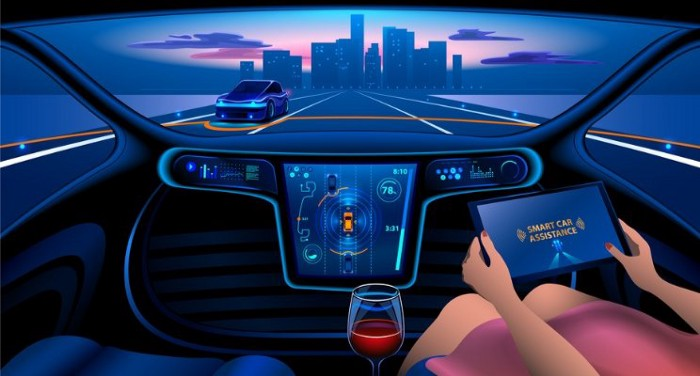
\includegraphics[scale=0.2]{imagenes/fiction}
%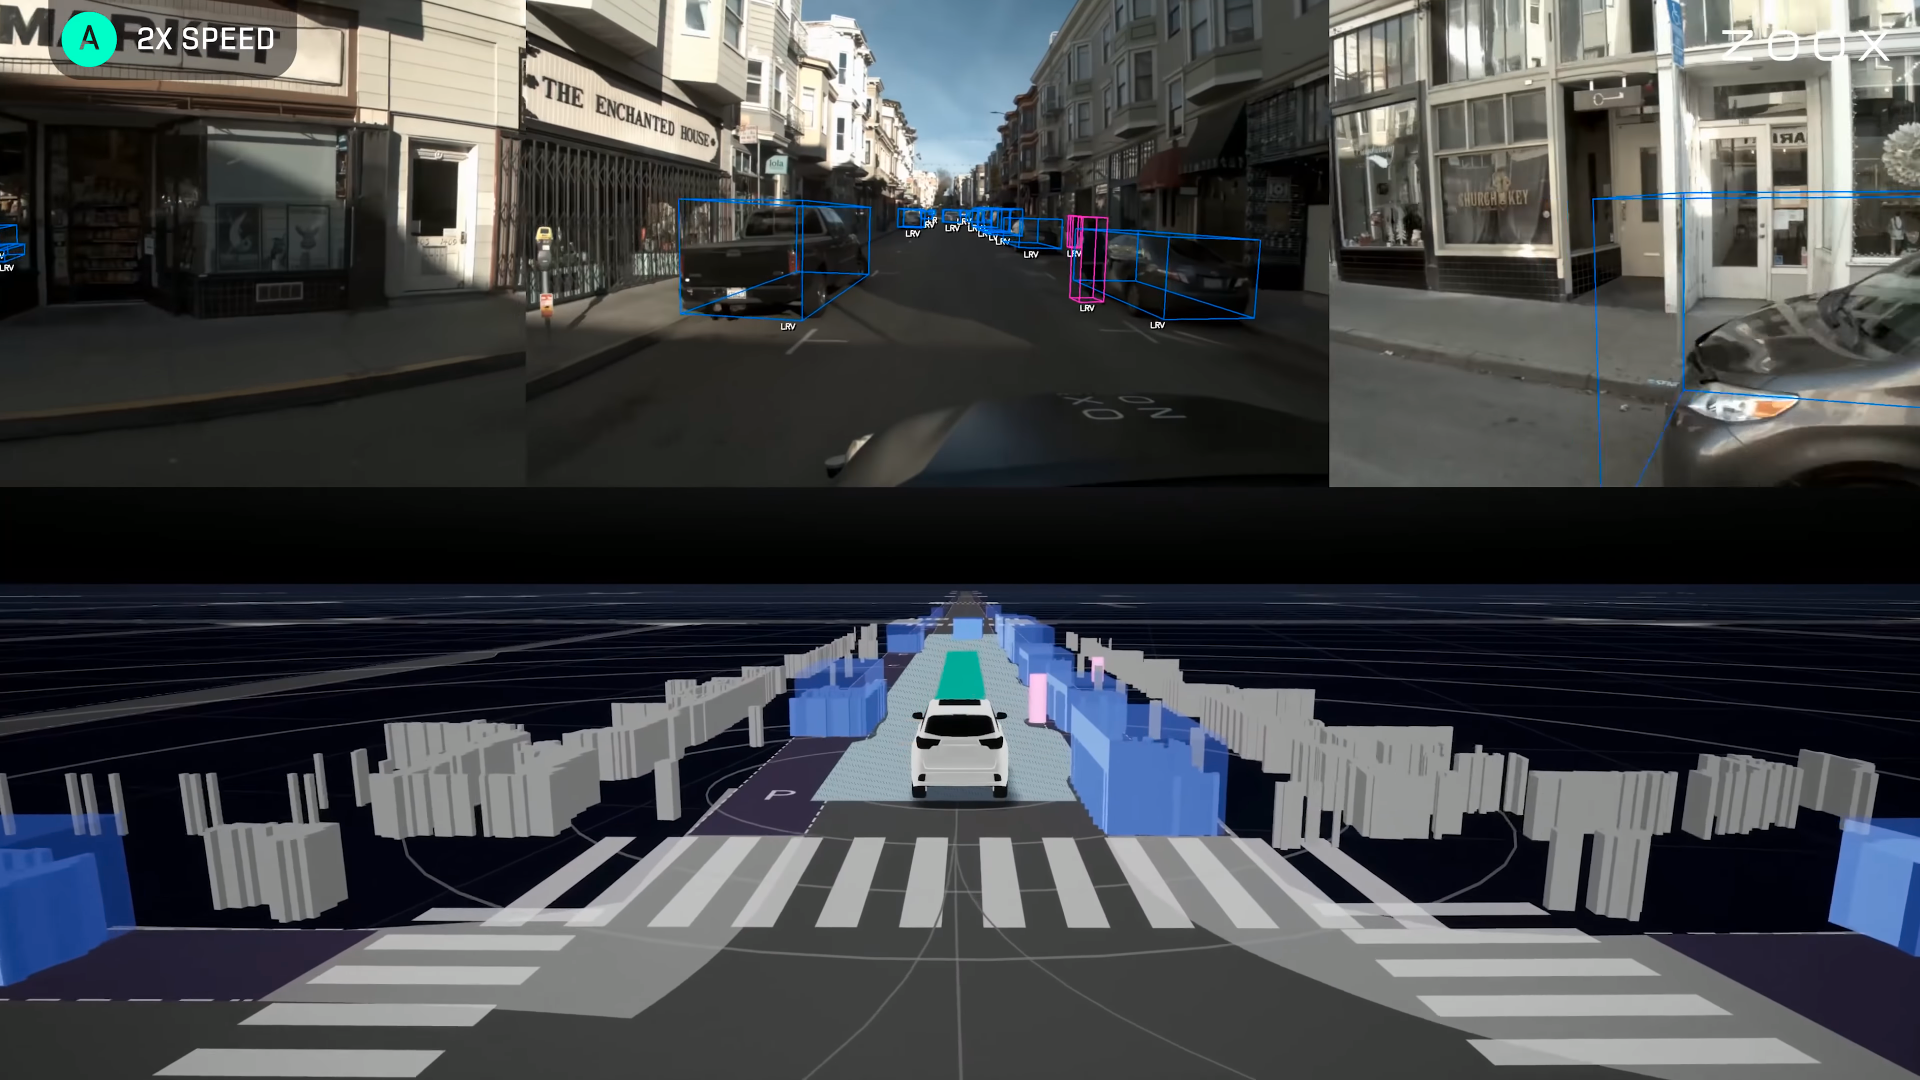
\includegraphics[scale=0.1]{imagenes/zoox}

\begin{figure}[H]
	\captionsetup[subfloat]{labelformat=empty}
	\centering
	\subfloat[][Ficción]{{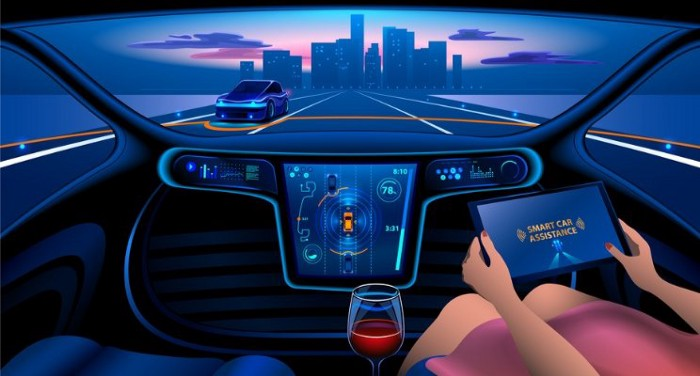
\includegraphics[width=5.3cm]{imagenes/fiction} }}%
	\subfloat[][Realidad]{{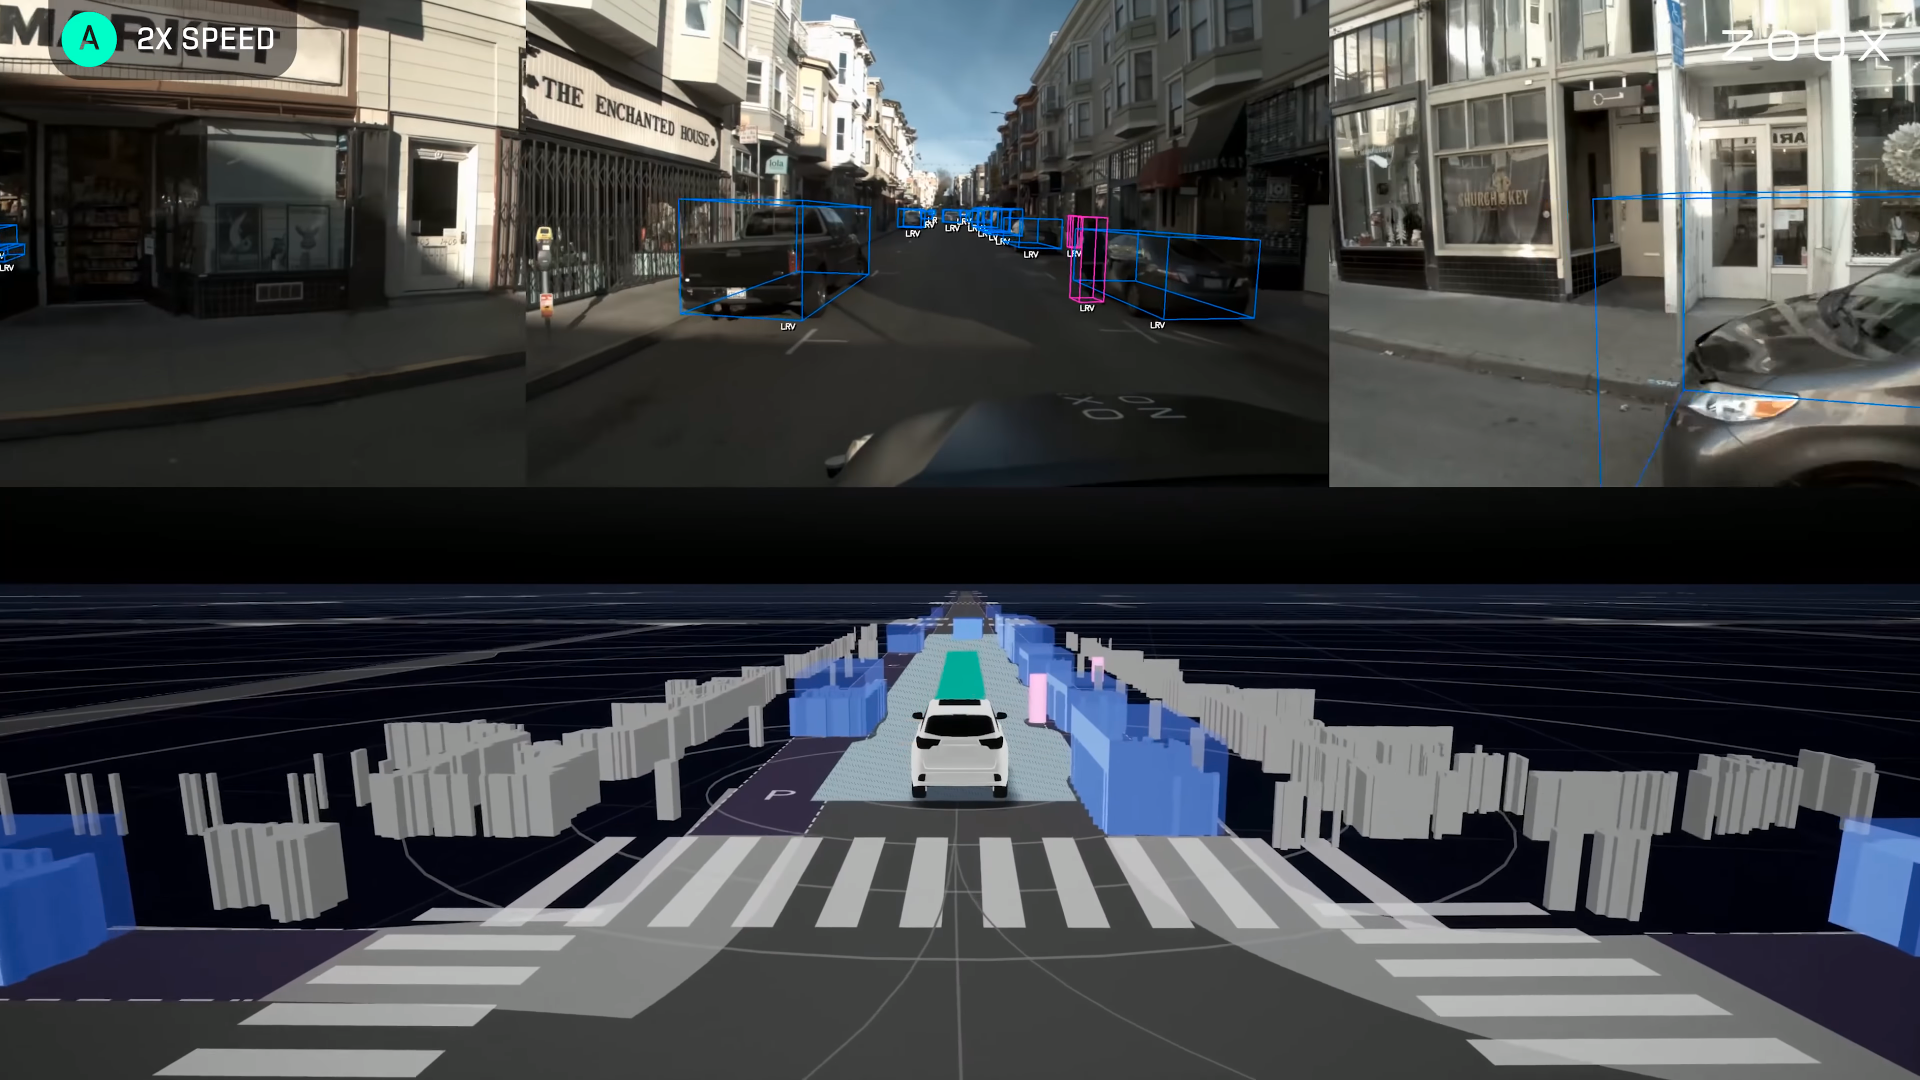
\includegraphics[width=5.1cm]{imagenes/zoox} }}%
\end{figure}

\begin{figure}[H]
	\captionsetup{labelformat=empty}
	\centering
	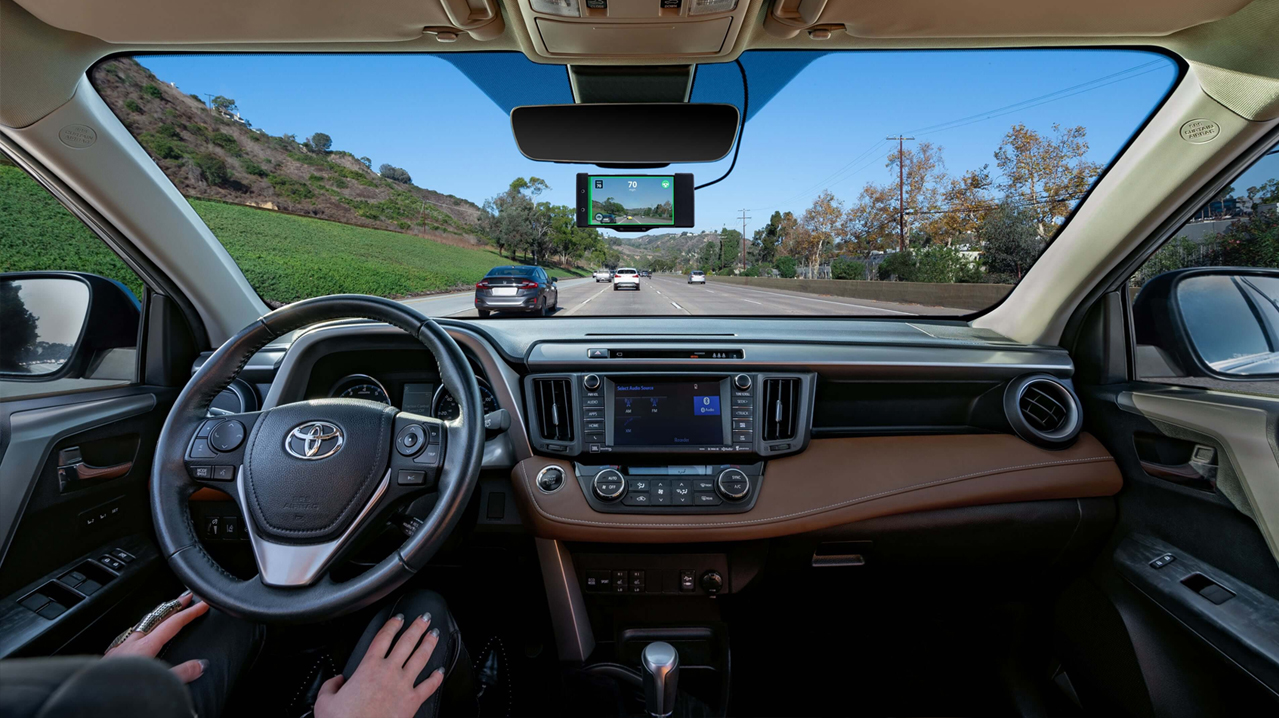
\includegraphics[width=5cm]{imagenes/comma}
	\caption{Propuestas Alternativas}
\end{figure}

\end{frame}

\begin{frame}[fragile]{Antecedentes}
	%	DARPA, DAVE, AUDI
	%	Lidar vs Pure CV
	\begin{figure}[H]
		\captionsetup[subfloat]{labelformat=empty}
		\centering
		\subfloat[][Dave]{{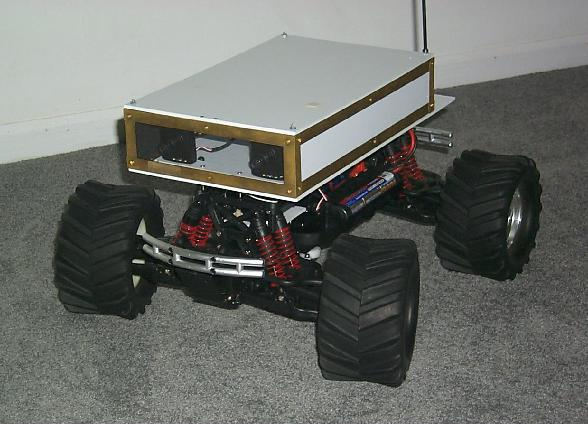
\includegraphics[width=3.5cm, valign=c]{imagenes/dave-1} }}%
		\subfloat[][Darpa Grand Challenge]{{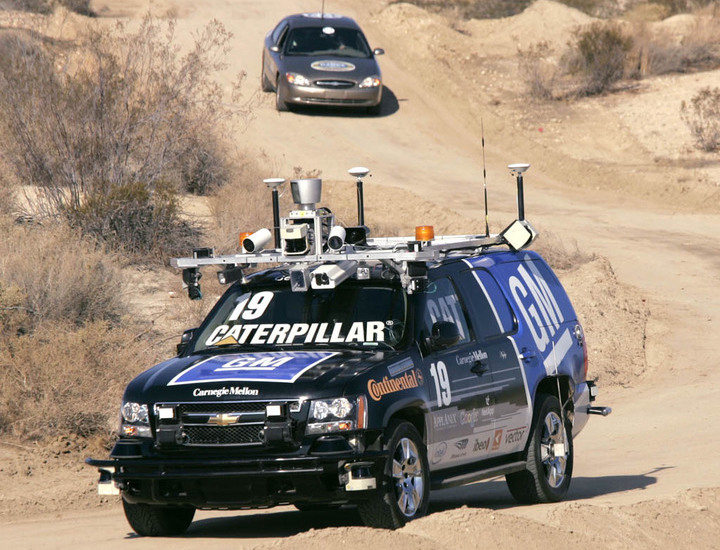
\includegraphics[width=3.5cm, valign=c]{imagenes/darpa} }}%
	\end{figure}
	
	\begin{figure}[H]
		\captionsetup{labelformat=empty}
		\centering
		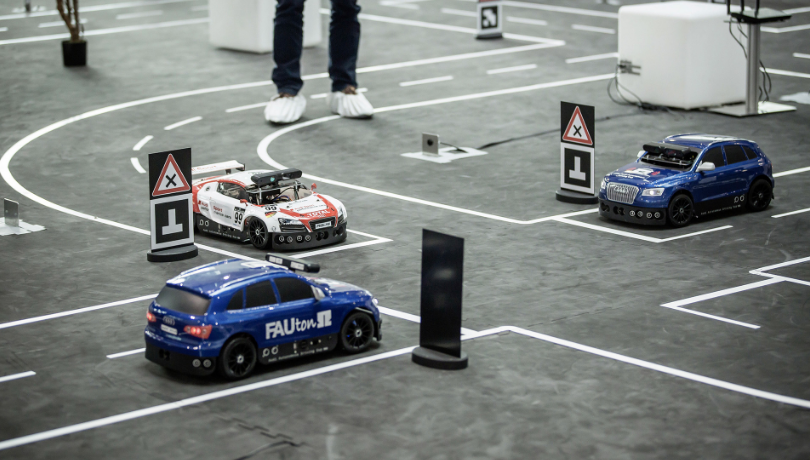
\includegraphics[width=4.5cm]{imagenes/audi}
		\caption{Competencias de vehículos a escala}
	\end{figure}
\end{frame}

\begin{frame}[fragile]{Objetivo General}
	\begin{center}
		\Large
		``Plantear un modelo para la conducción autónoma que logre una autonomía básica en vías de doble sentido con separación física''
	\end{center}
\end{frame}

\begin{frame}[fragile]{Objetivos Específicos}
	\begin{itemize}[<+-|alert@+>]
		\item Diseñar un componente de aumentación y preprocesamiento de datos para extraer y crear un dataset con el fin de resolver la tarea.
		\item Reducir la complejidad de implementación del modelo mediante el uso de solamente una cámara.
		\item Modificar y entrenar redes neuronales con una alta exactitud en las predicciones utilizando menos requisitos de cómputo.
	\end{itemize}
\end{frame}


\begin{frame}[fragile]{Objetivos Específicos}
	\begin{itemize}[<+-|alert@+>]
		\item Analizar las predicciones de los modelos entrenados para comprobar si las representaciones aprendidas son invariantes a los cambios de perspectiva, iluminación y objetos en la imagen.
		\item Combinar las salidas de algoritmos de visión computacional y modelos de aprendizaje profundo para mejorar la generalización de predicciones.
		\item Probar el rendimiento del modelo en una simulación, analizando casos de fallas y qué situaciones puede manejar correctamente.
	\end{itemize}
\end{frame}

\begin{frame}[fragile]{Hipótesis}
	\begin{center}
		\Large
		``El modelo de conducción autónoma mediante el uso de aprendizaje profundo y algoritmos de visión computacional alcanza una autonomía de nivel 2 en vías de doble sentido con separación física''
	\end{center}
\end{frame}

\begin{frame}[fragile]{Justificación}
	\begin{figure}[H]
		\captionsetup[subfloat]{labelformat=empty}
		\centering
		\subfloat[][Económica]{{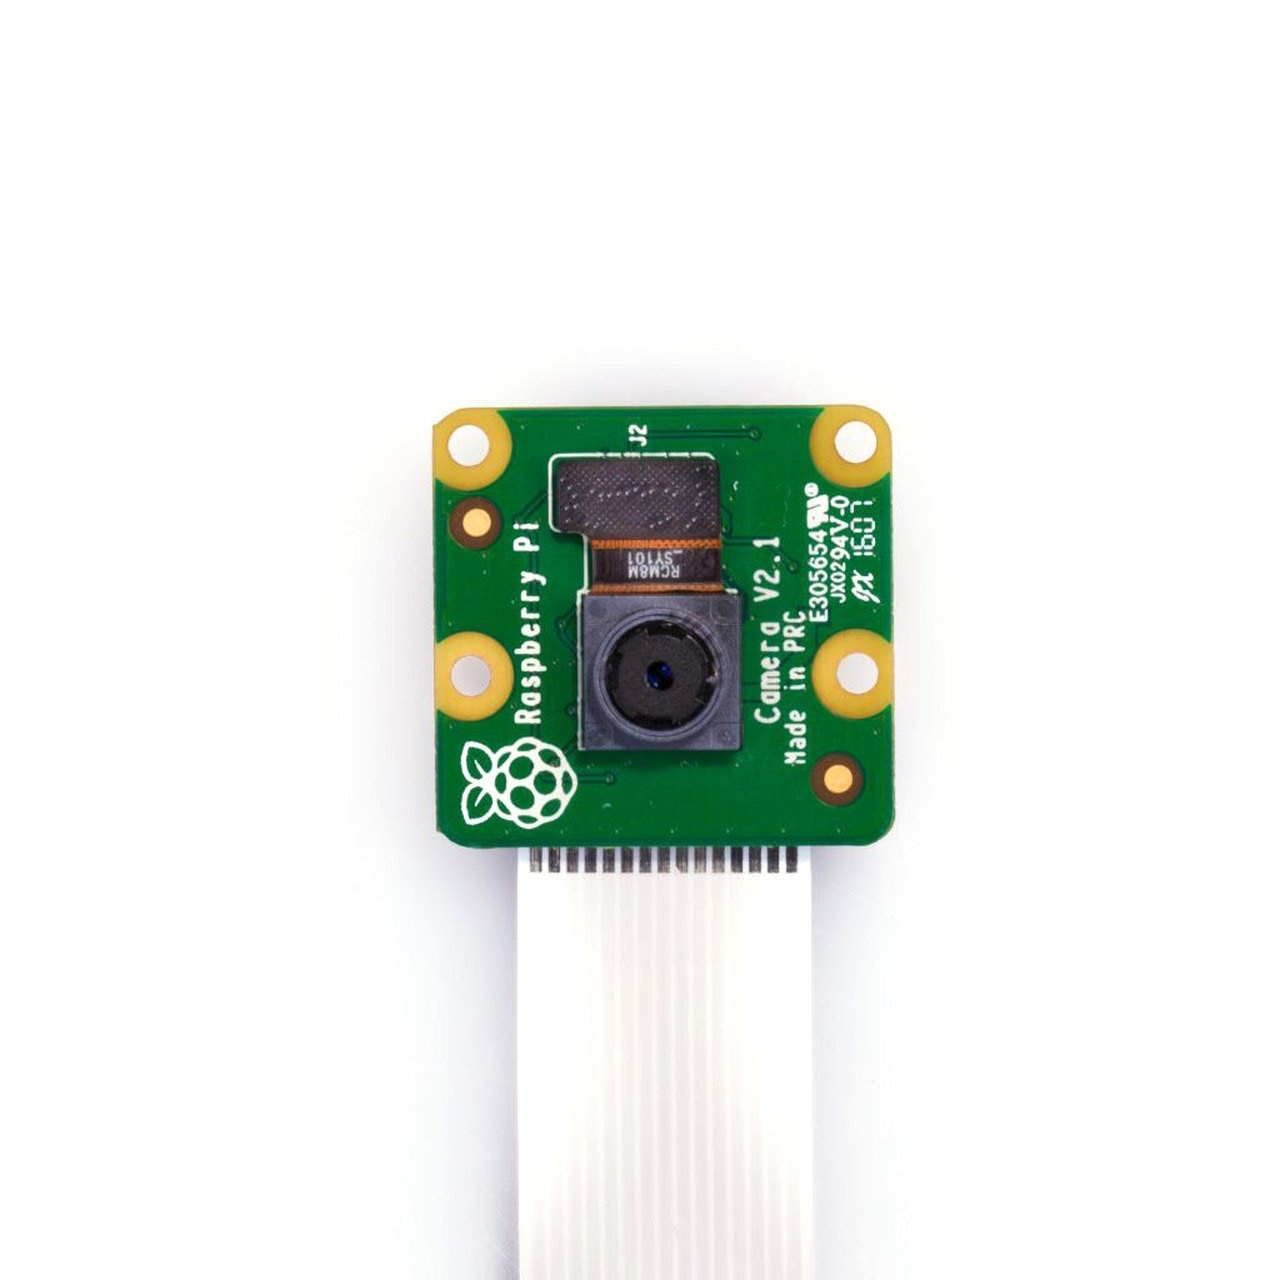
\includegraphics[width=3cm]{imagenes/cam} }}
		\subfloat[][Social]{{
\includegraphics[width=3cm]{imagenes/octocat} }}
		\subfloat[][Científica]{{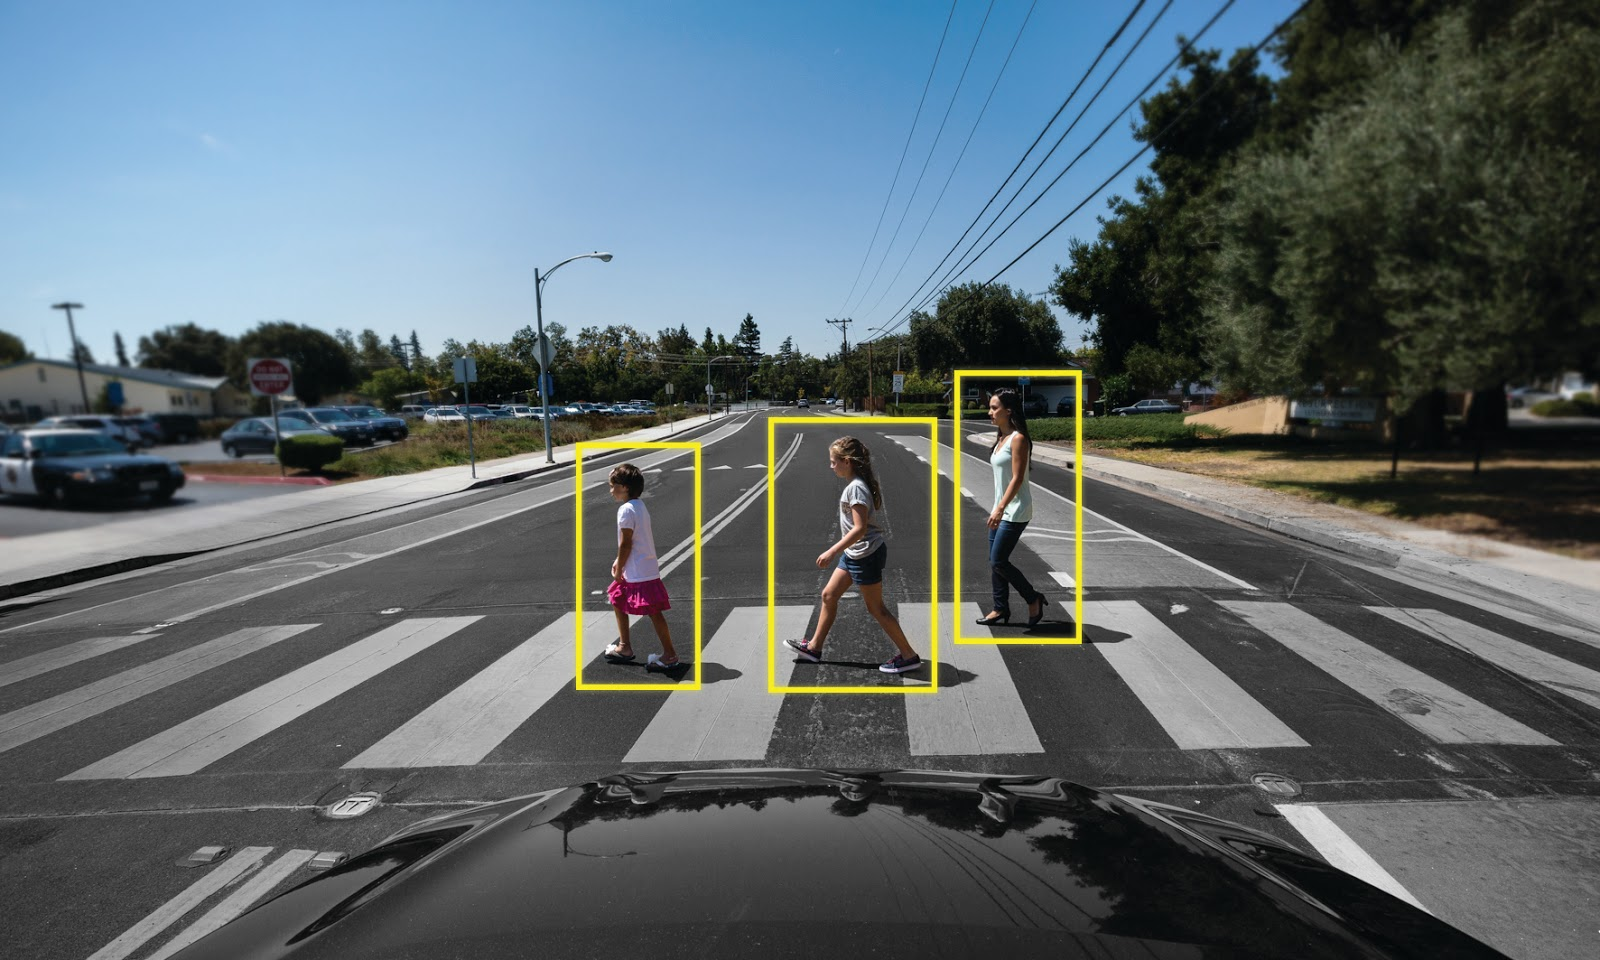
\includegraphics[width=3.5cm]{imagenes/obj_det} }}
	\end{figure}
\end{frame}

\begin{frame}[fragile]{Alcances}
	\begin{figure}[H]
		\captionsetup[subfloat]{labelformat=empty}
		\centering
		\subfloat{{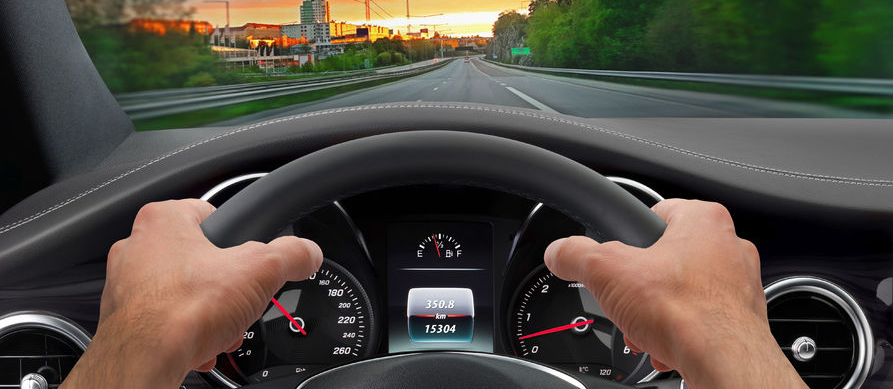
\includegraphics[width=5cm, valign=c]{imagenes/steering} }}
		\subfloat{{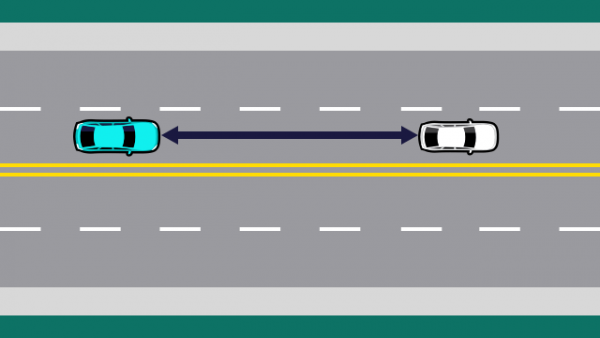
\includegraphics[width=4.5cm, valign=c]{imagenes/distance} }}
	\end{figure}

	\begin{figure}[H]
		\captionsetup{labelformat=empty}
		\centering
		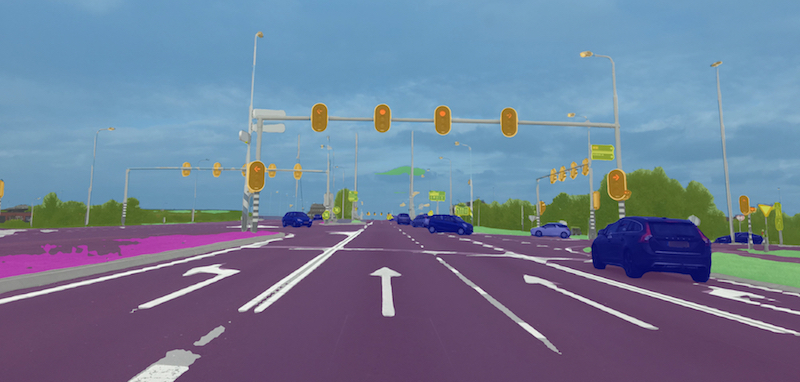
\includegraphics[width=6cm]{imagenes/semseg1}
	\end{figure}
\end{frame}

\begin{frame}[fragile]{Límites}
%	lidar
%	path planning
%	Doble sentido
%	No lluvia extrema

	\begin{figure}[H]
		\captionsetup[subfloat]{labelformat=empty}
		\centering
		\subfloat{{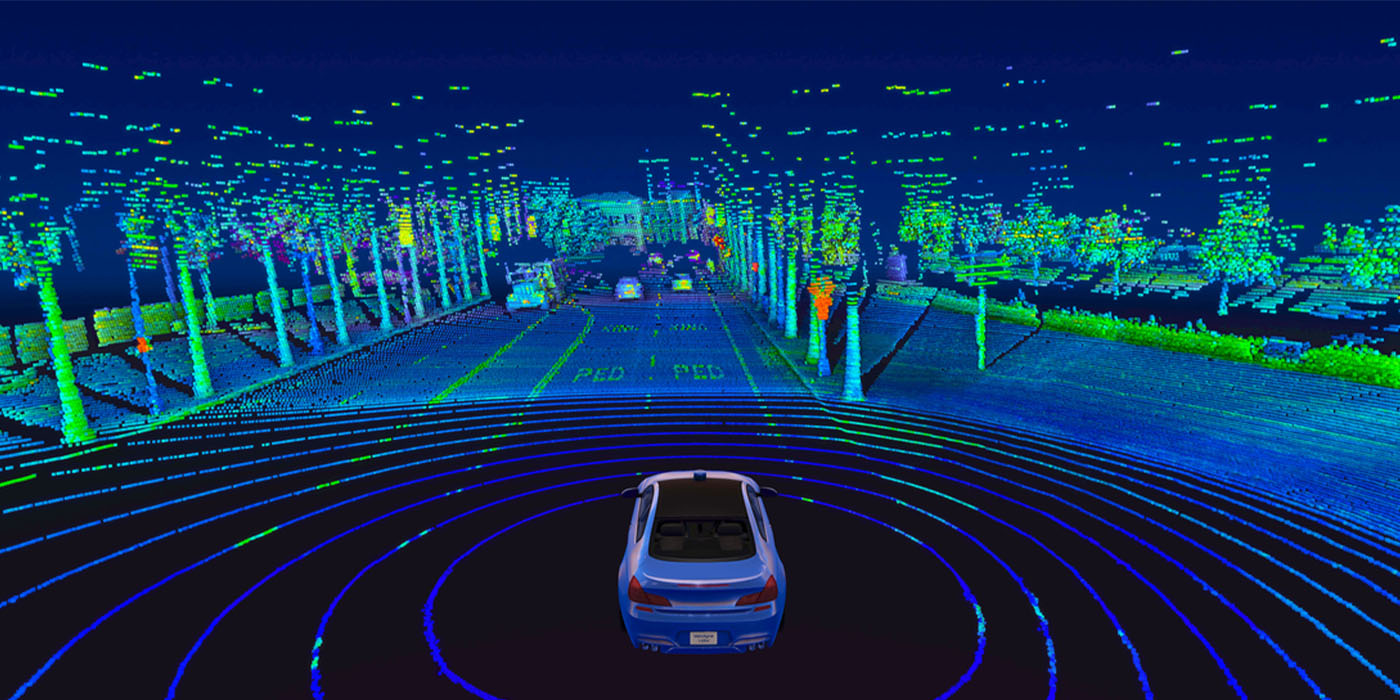
\includegraphics[width=5cm, valign=c]{imagenes/lidar} }}
		\subfloat{{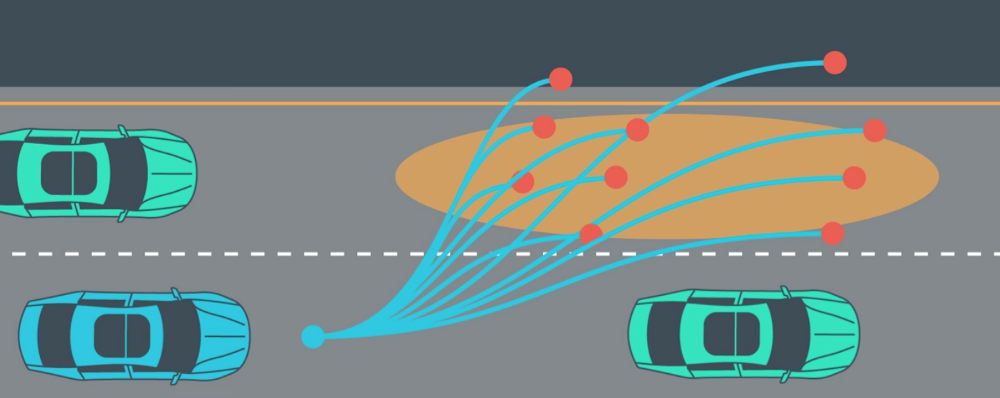
\includegraphics[width=4.5cm, valign=c]{imagenes/path} }}
	\end{figure}

	\begin{figure}[H]
		\captionsetup[subfloat]{labelformat=empty}
		\centering
		\subfloat{{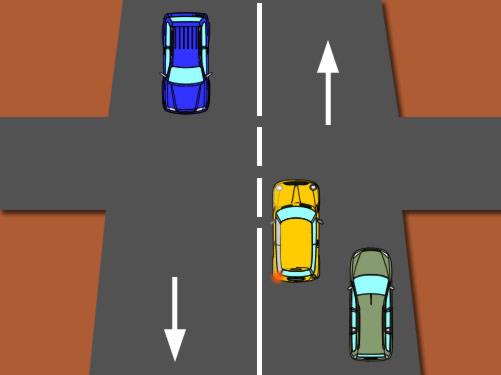
\includegraphics[width=5cm, valign=c]{imagenes/doblevia} }}
		\subfloat{{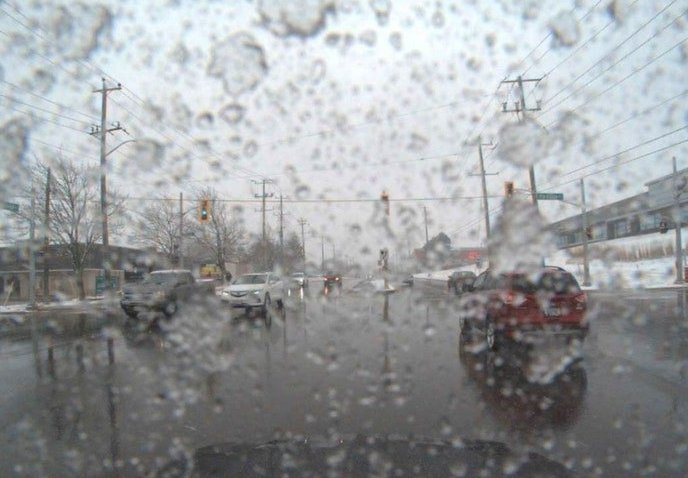
\includegraphics[width=4.5cm, valign=c]{imagenes/lluvia} }}
	\end{figure}
\end{frame}

\begin{frame}[fragile]{Metodología}
	\begin{figure}[H]
		\captionsetup[subfloat]{labelformat=empty}
		\centering
		\subfloat{{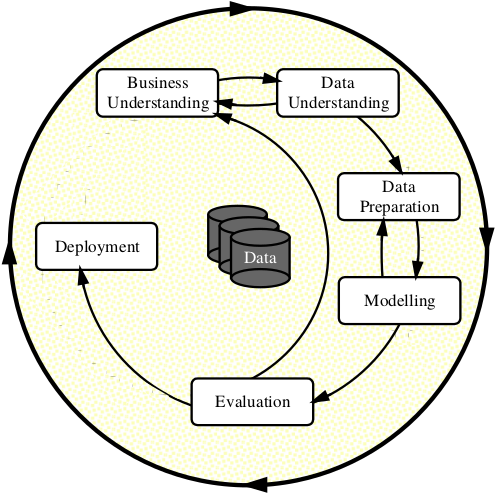
\includegraphics[width=4cm, valign=c]{imagenes/crisp} }}
		\hspace{2mm}
		\subfloat{{
\includegraphics[width=5cm, valign=c]{imagenes/ibm} }}
	\end{figure}
\end{frame}

\section[MARCO TEÓRICO]{Marco Teórico}
\begin{frame}[fragile]{Sistemas de Conducción Autónoma}
	\begin{figure}[H]
		\captionsetup[subfloat]{labelformat=empty}
		\centering
		\subfloat{{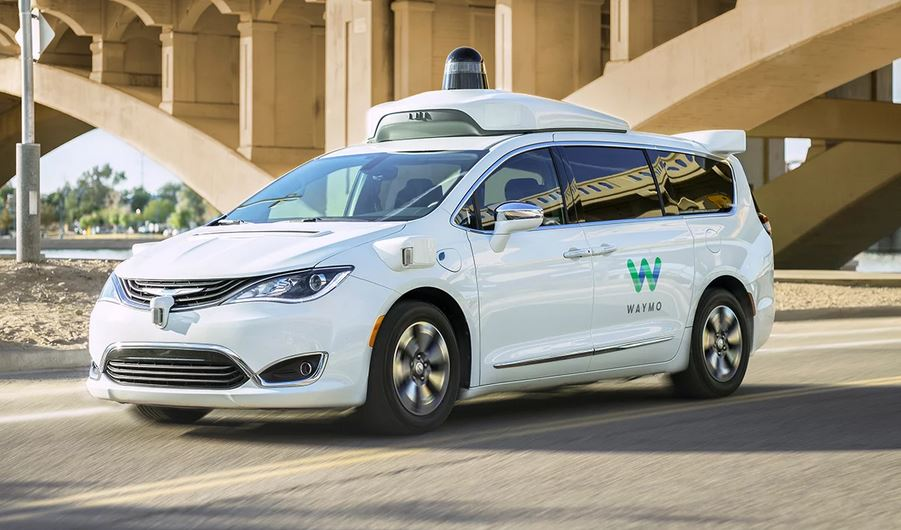
\includegraphics[width=5cm, valign=c]{imagenes/waymo} }}
		\subfloat{{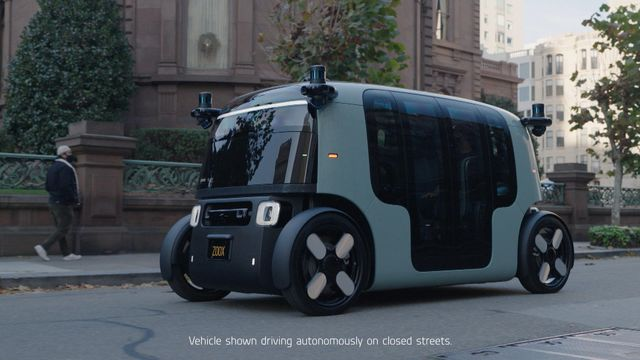
\includegraphics[width=5.1cm, valign=c]{imagenes/zoox2} }}
	\end{figure}
	
	\begin{figure}[H]
		\captionsetup{labelformat=empty}
		\centering
		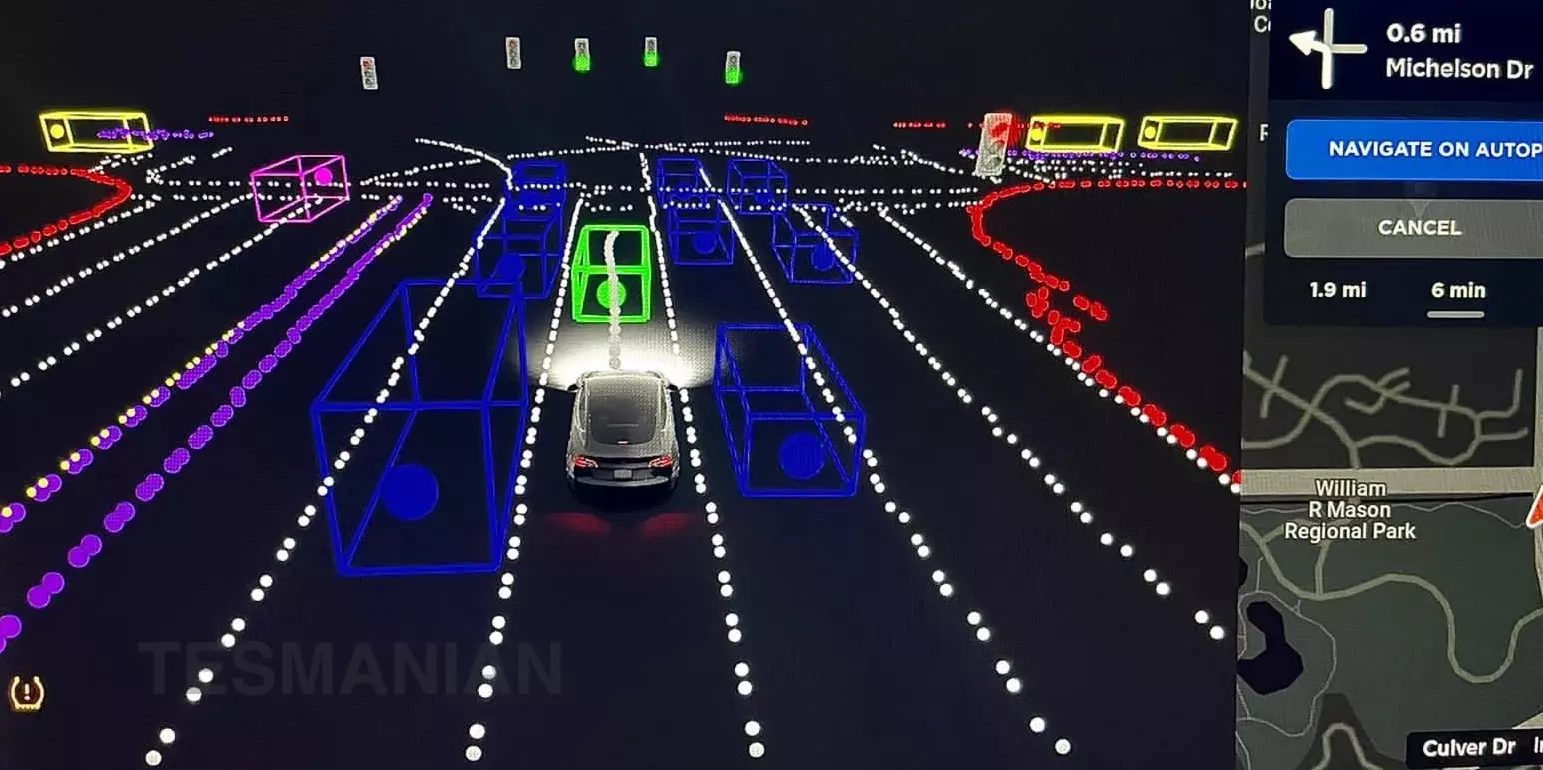
\includegraphics[width=7cm]{imagenes/tesla}
	\end{figure}
\end{frame}

\begin{frame}[fragile]{Visión Computacional}
%	Imagen, Conv
	\begin{figure}[H]
		\captionsetup[subfloat]{labelformat=empty}
		\centering
		\subfloat{{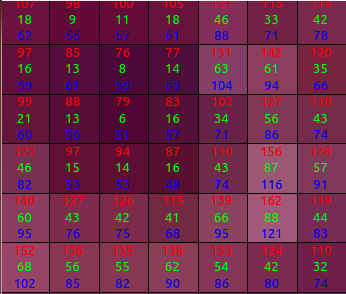
\includegraphics[width=5cm, valign=c]{imagenes/pixels2} }}
		\hspace{2mm}
		\subfloat{{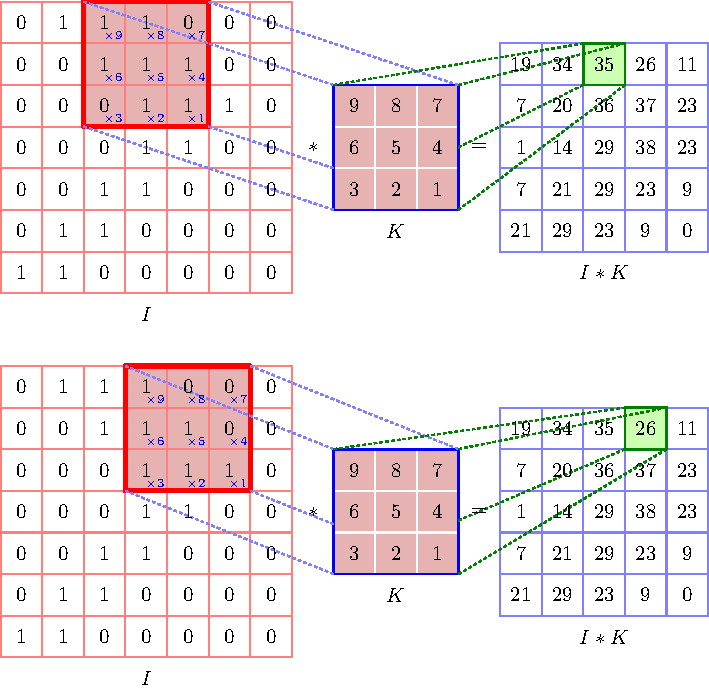
\includegraphics[width=5.1cm, valign=c]{imagenes/conv1} }}
	\end{figure}
\end{frame}

\begin{frame}[fragile]{Visión Computacional}
%	Dilatacion, erosion, apertura
	\begin{figure}[H]
		\captionsetup[subfloat]{labelformat=empty}
		\centering
		\subfloat{{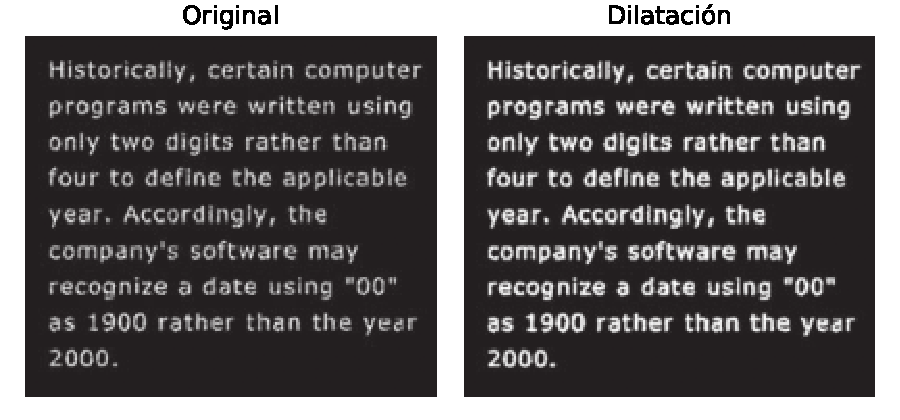
\includegraphics[width=5.3cm, valign=c]{imagenes/dilatacion} }}
		\subfloat{{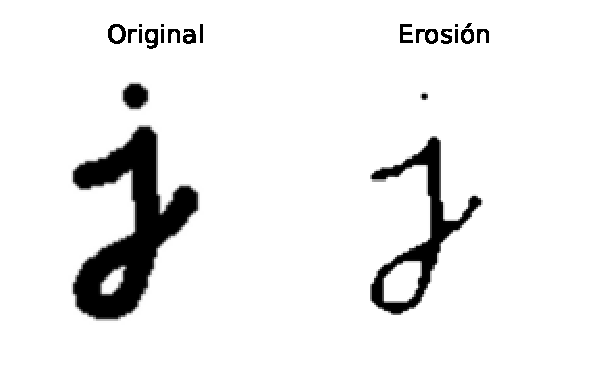
\includegraphics[width=5cm, valign=c]{imagenes/erosion} }}
	\end{figure}
	
	\begin{figure}[H]
		\captionsetup{labelformat=empty}
		\centering
		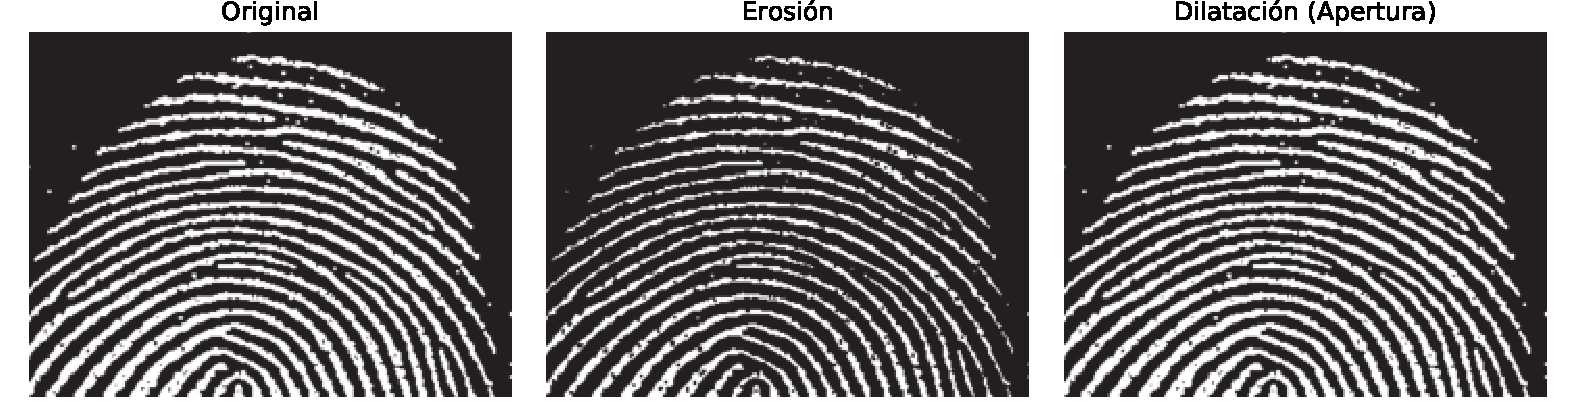
\includegraphics[width=10cm]{imagenes/apertura}
	\end{figure}
\end{frame}

\begin{frame}[fragile]{Visión Computacional}
%	Flood Fill y K Means
	\begin{figure}[H]
		\captionsetup[subfloat]{labelformat=empty}
		\centering
		\subfloat{{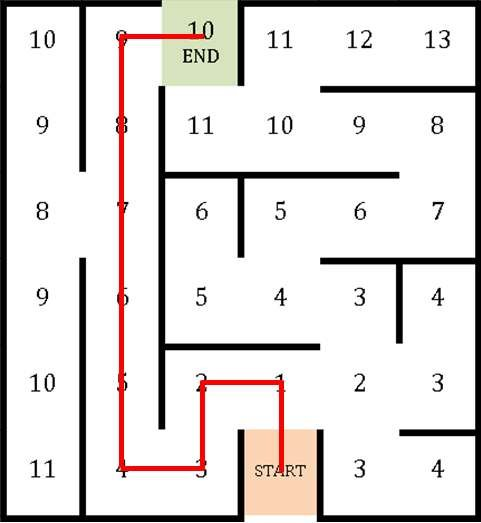
\includegraphics[width=4.3cm, valign=c]{imagenes/ff} }}
		\hspace{2mm}
		\subfloat{{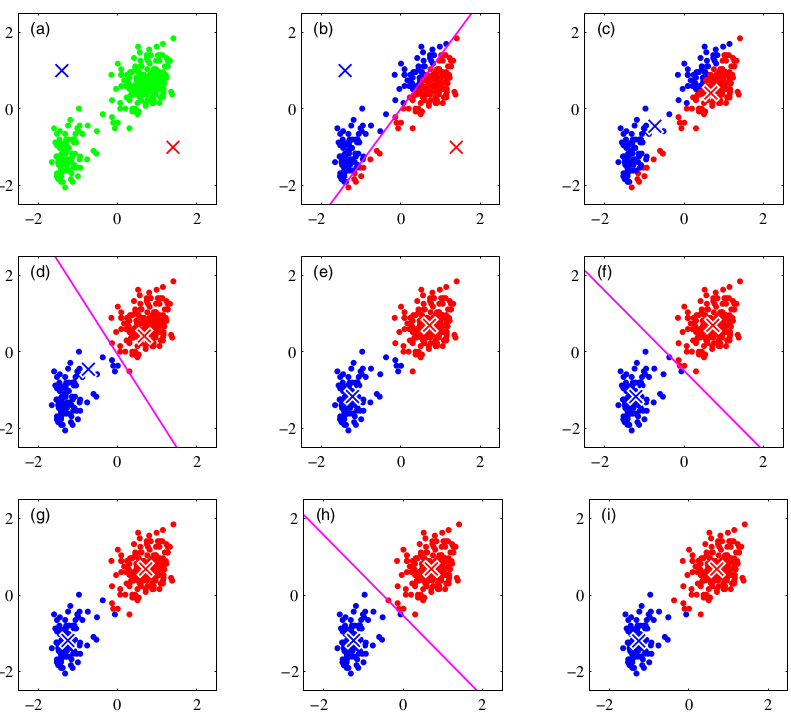
\includegraphics[width=5.5cm, valign=c]{imagenes/kmeans} }}
	\end{figure}
\end{frame}

\begin{frame}[fragile]{Visión Computacional}
	\begin{figure}[H]
		\captionsetup{labelformat=empty}
		\centering
		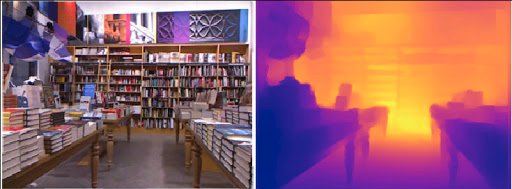
\includegraphics[width=8cm]{imagenes/depth2}
	\end{figure}
	
	\begin{figure}[H]
		\captionsetup{labelformat=empty}
		\centering
		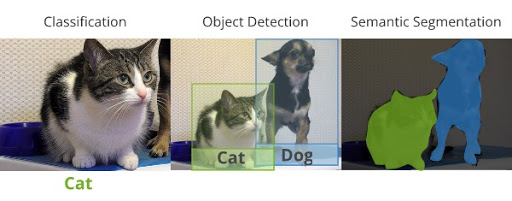
\includegraphics[width=10cm]{imagenes/obj}
	\end{figure}
\end{frame}

\begin{frame}[fragile]{Aprendizaje Automático}
%	Regresion y generalizada
	\begin{figure}[H]
		\captionsetup[subfloat]{labelformat=empty}
		\centering
		\subfloat{{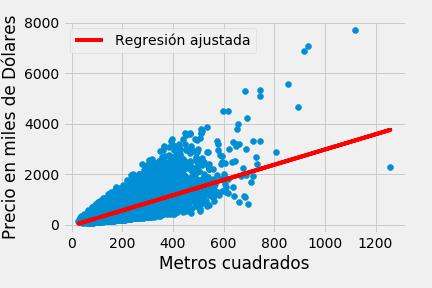
\includegraphics[width=5.1cm]{imagenes/linear_fit} }}
		\hspace{2mm}
		\subfloat{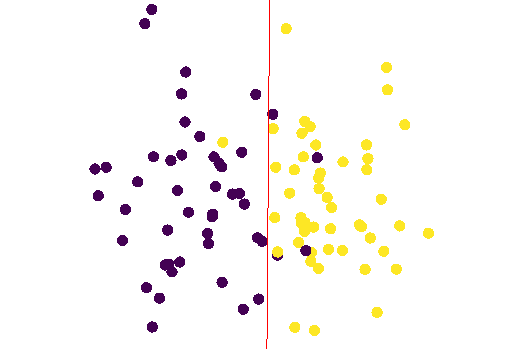
\includegraphics[width=5cm]{imagenes/logistic_reg}}
	\end{figure}

	$$Softmax(Z) = \frac{e^{Z}}{\sum_{j=1}^{C} e^{Z_j}}$$
\end{frame}

\begin{frame}[fragile]{Aprendizaje Profundo}
%	NN, SGD
	\begin{figure}[H]
		\captionsetup[subfloat]{labelformat=empty}
		\centering
		\subfloat{{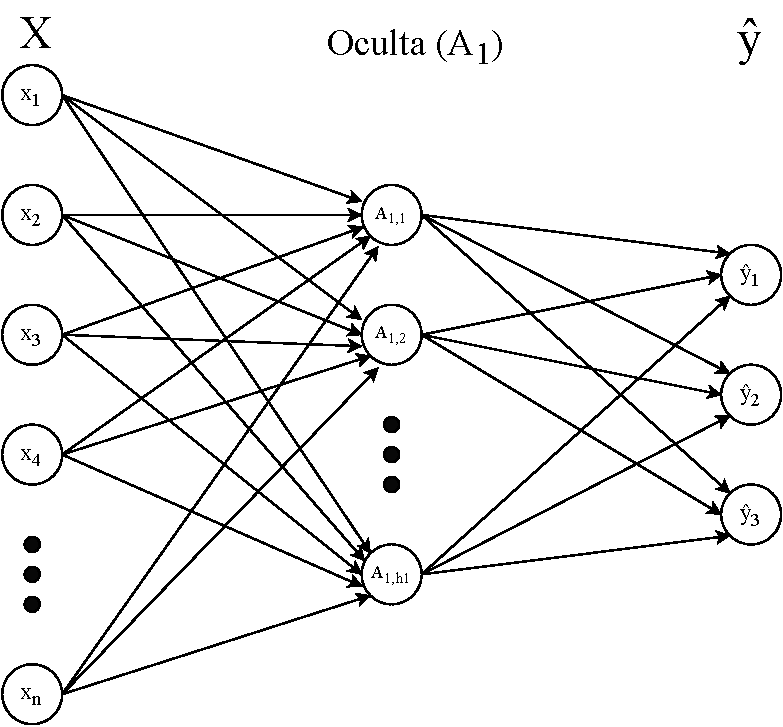
\includegraphics[width=4cm, valign=c]{imagenes/NeuralNetwork} }}
		\hspace{2mm}
		\subfloat{{\visible<2->{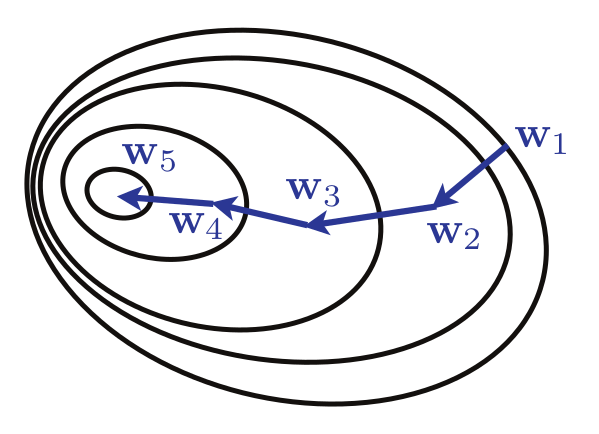
\includegraphics[width=4cm, valign=c]{imagenes/sgd} }}}
			
		\visible<3->{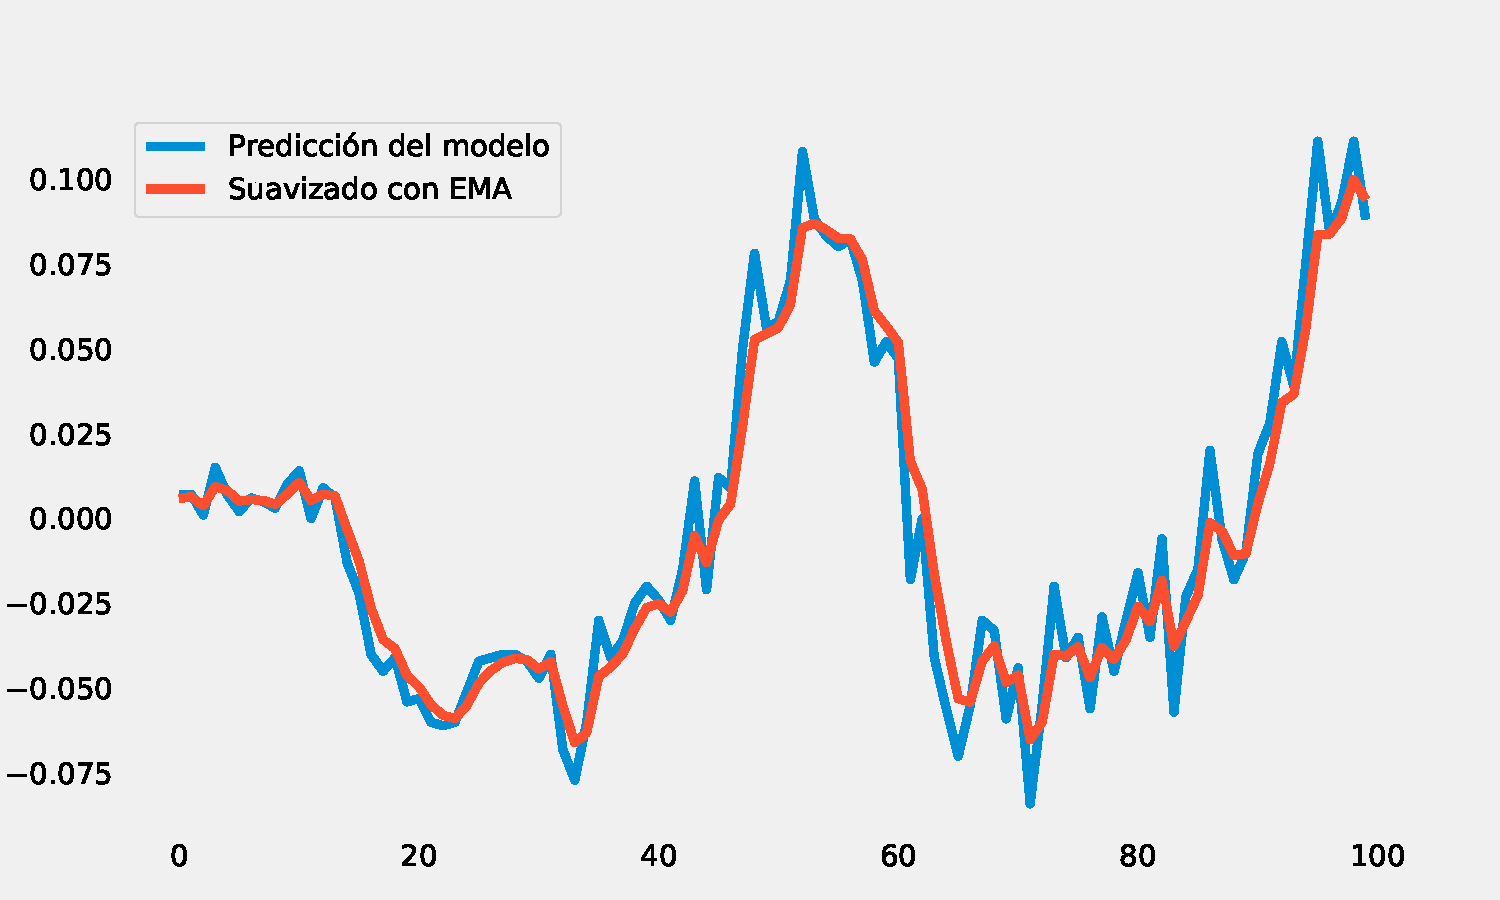
\includegraphics[width=6cm]{imagenes/ema}}
	\end{figure}
\end{frame}

\begin{frame}[fragile]{Redes Convolucionales}
%	CNN, MOBILENET, FastDepth
	\begin{figure}[H]
		\captionsetup[subfloat]{labelformat=empty}
		\centering
		\subfloat{{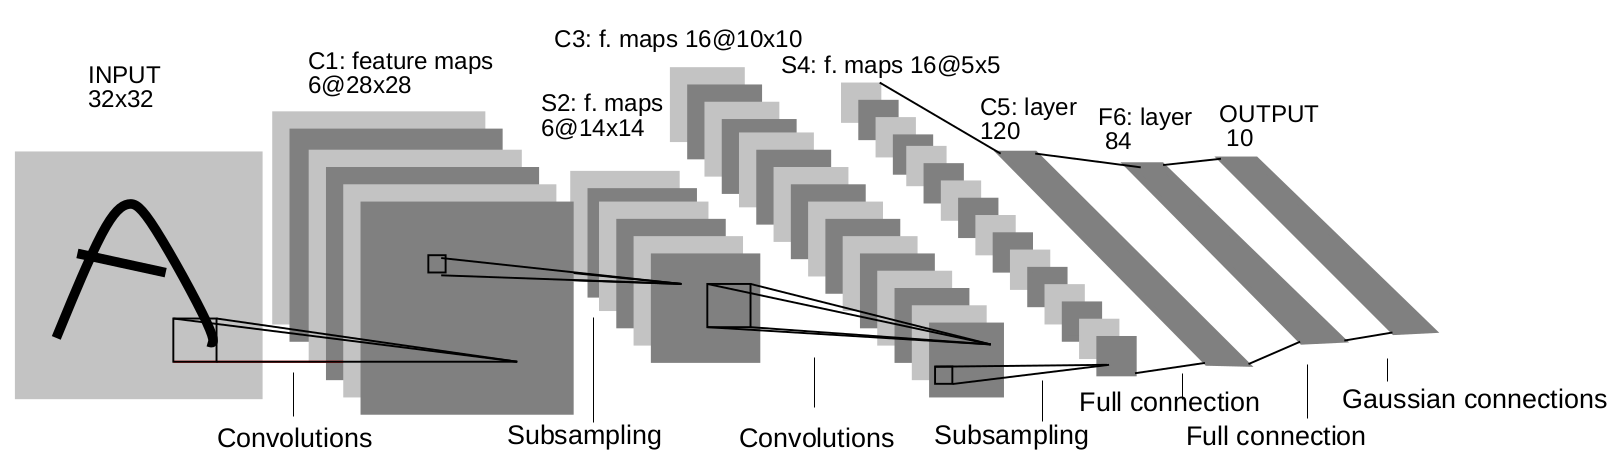
\includegraphics[width=5.5cm, valign=c]{imagenes/lenet} }}
		\subfloat{{\visible<2->{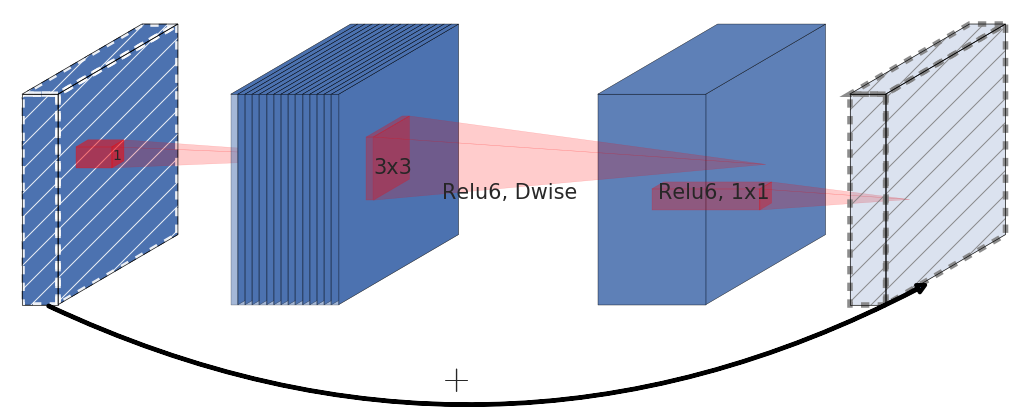
\includegraphics[width=5.5cm, valign=c]{imagenes/bottleneck} }}}
	\end{figure}
	\visible<3->{
	\begin{figure}[H]
		\captionsetup{labelformat=empty}
		\centering
		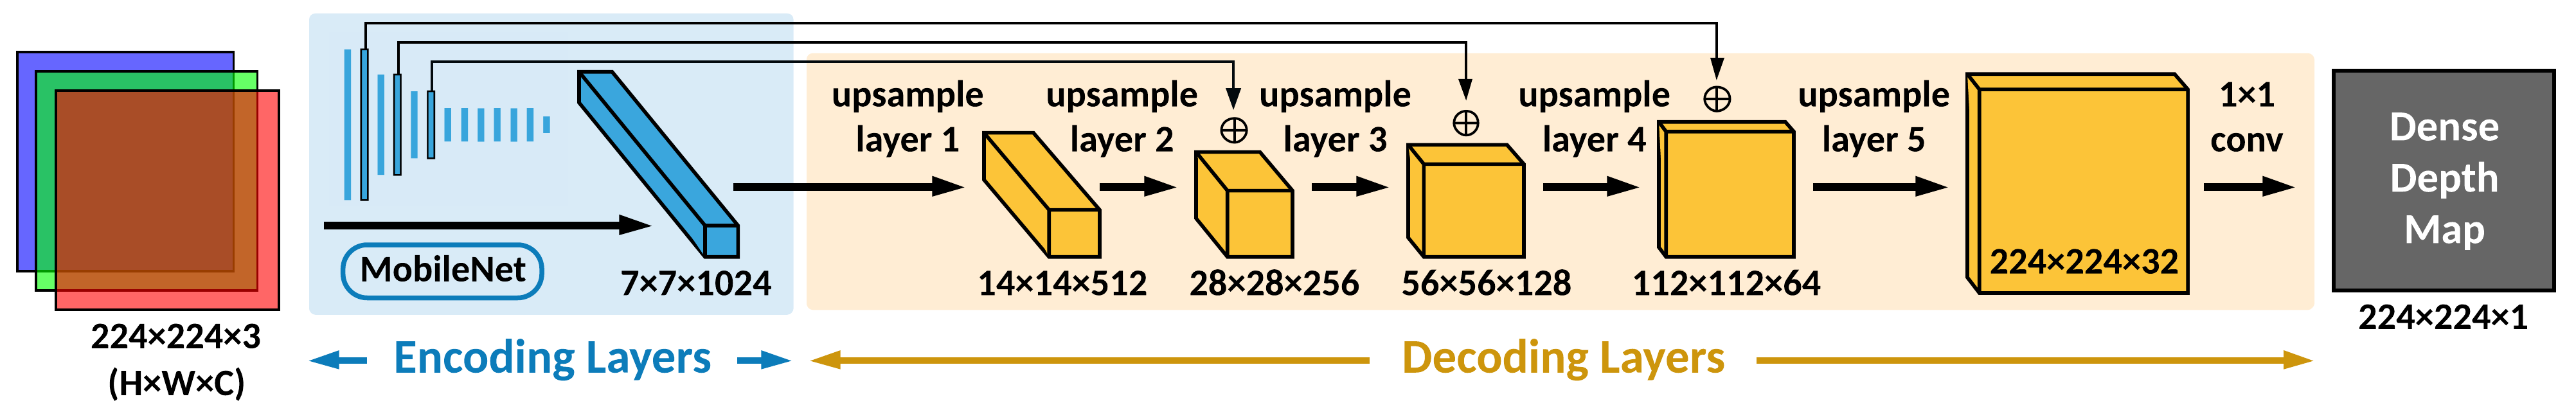
\includegraphics[height=1.7cm]{imagenes/fastdepth}
	\end{figure}}
\end{frame}

\begin{frame}[fragile]{SCORECAM}
	\begin{figure}[H]
		\captionsetup{labelformat=empty}
		\centering
		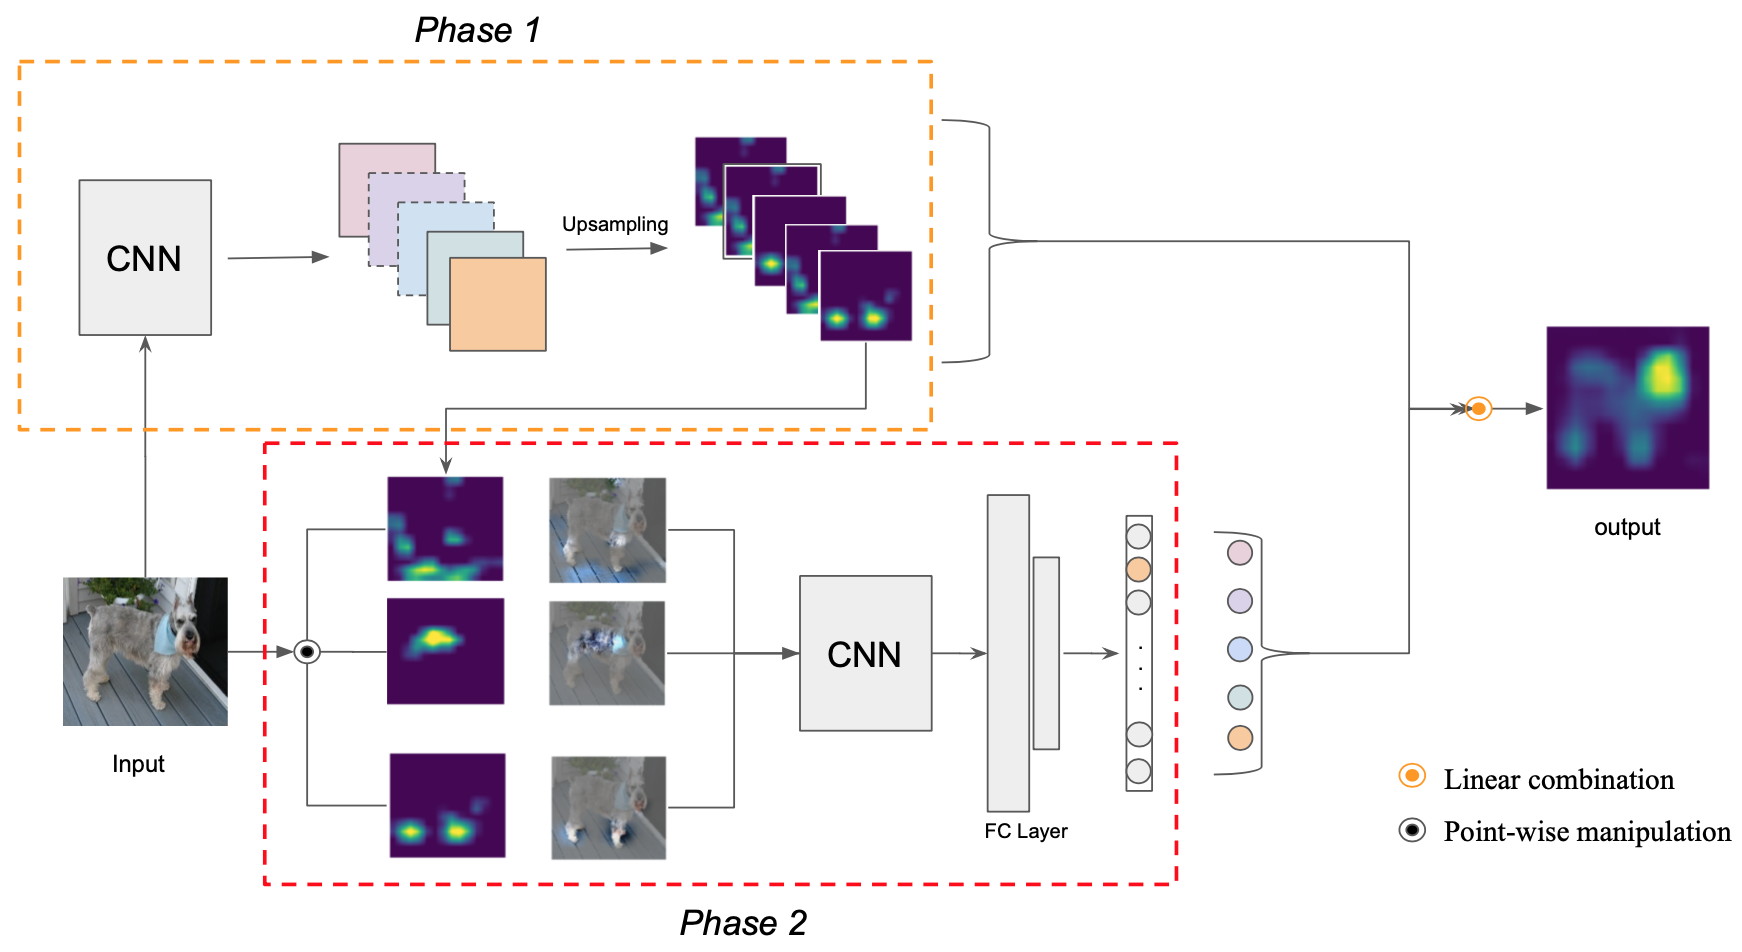
\includegraphics[height=6cm]{imagenes/scorecam_net}
	\end{figure}
\end{frame}

\begin{frame}[fragile]{Métricas de Error}
	
	\begin{multicols}{3}
		$$MSE = \frac{1}{n}\sum_{i=1}^n (\hat{y} - y)^2$$
		$$MAE = \frac{1}{n}\sum_{i=1}^n |\hat{y} - y|$$
		\break
		\visible<2->{
		$$P = \frac{T_p}{T_p + F_p}$$		
		$$R = \frac{T_p}{T_p + F_n}$$		
		$$F = 2\frac{P\cdot R}{P+R}$$}
		\break
		\visible<3->{
		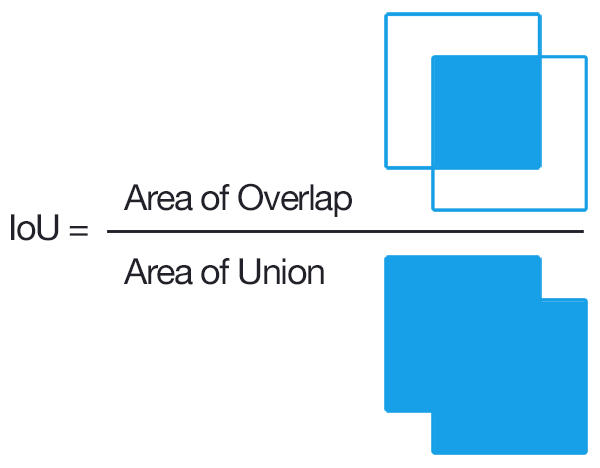
\includegraphics[height=3cm]{imagenes/iou}}
	\end{multicols}
	
\end{frame}

%\begin{frame}[fragile]{Métricas de Error}
%	%	IOU
%%	$$IoU = \frac{|y\cap\hat{y}|}{|y\cup\hat{y}|}$$
%	
%	\begin{figure}[H]
%		\captionsetup{labelformat=empty}
%		\centering
%		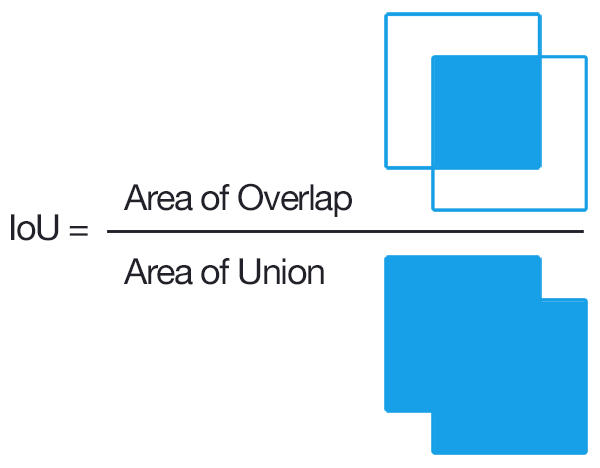
\includegraphics[height=5cm]{imagenes/iou}
%	\end{figure}
%\end{frame}

\section[MARCO APLICATIVO]{Marco Aplicativo}
\begin{frame}[fragile]{Estructura del Proyecto}
%	Etapas
	\begin{figure}[H]
		\captionsetup{labelformat=empty}
		\centering
		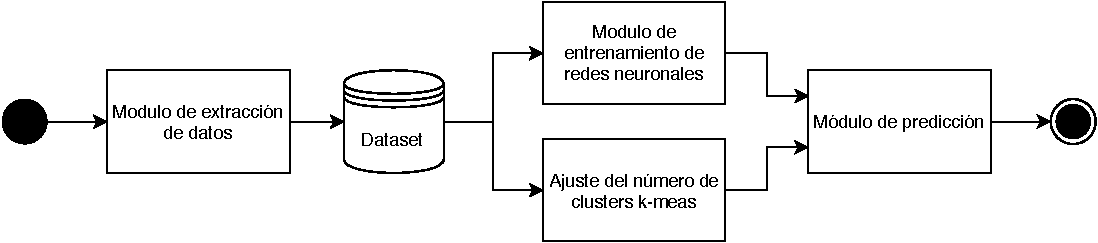
\includegraphics[width=10cm]{imagenes/arquitectura_proyecto}
	\end{figure}
\end{frame}

\begin{frame}[fragile]{Extracción de datos}
%   Módulo de extracción
	\begin{figure}[H]
		\captionsetup{labelformat=empty}
		\centering
		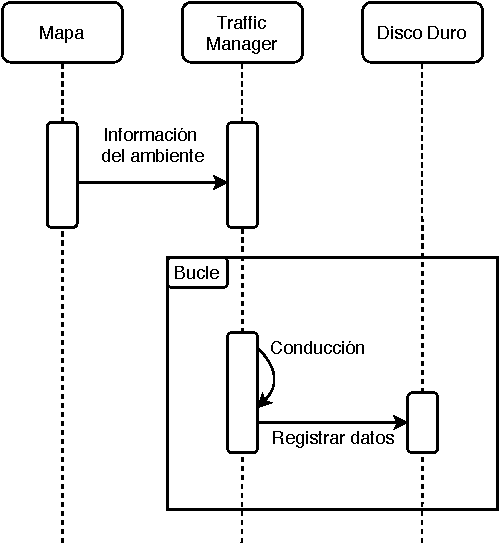
\includegraphics[width=5cm]{imagenes/arquitectura-extraccion}
	\end{figure}
\end{frame}

\begin{frame}[fragile]{Profundidad}
%	Preprocesamiento y límite 30
	\begin{figure}[H]
		\captionsetup{labelformat=empty}
		\centering
		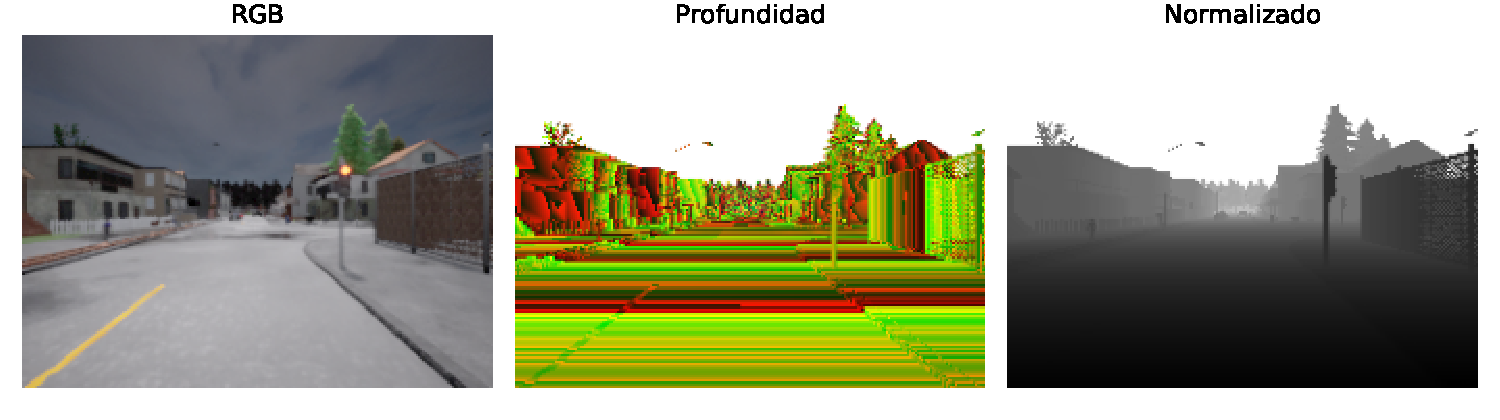
\includegraphics[width=10cm]{imagenes/depth}
	\end{figure}
\end{frame}

\begin{frame}[fragile]{Segmentación}
%	Pre Procesamiento de la segmentación y clases
	\begin{figure}[H]
		\captionsetup{labelformat=empty}
		\centering
		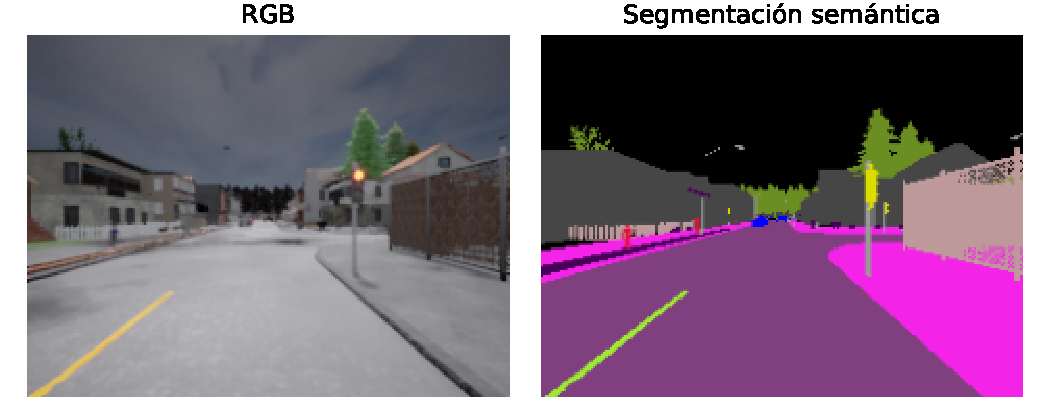
\includegraphics[width=10cm]{imagenes/semseg}
	\end{figure}
\end{frame}

%\begin{frame}[fragile]{Intersecciones}
%%	Etiquetado y unión total de los DF
%\end{frame}
%
\begin{frame}[fragile]{Entrenamiento de las Redes Neuronales}
%	Cascada 3 redes
	\begin{figure}[H]
		\captionsetup{labelformat=empty}
		\centering
		\includegraphics[width=10cm]{imagenes/arquitectura_entrenamiento}
	\end{figure}
\end{frame}
%
\begin{frame}[fragile]{DriveNet}
	\begin{figure}[H]
		\captionsetup{labelformat=empty}
		\centering
		\includegraphics[width=10cm]{imagenes/drivenet}
	\end{figure}
\end{frame}

\begin{frame}[fragile]{DepthNet y SemsegNet}
	\begin{figure}[H]
		\captionsetup[subfloat]{labelformat=empty}
		\centering
		\subfloat{{\includegraphics[width=5cm, valign=c]{imagenes/depthnet} }}
		\hspace{2mm}
		\subfloat{{\includegraphics[width=5cm, valign=c]{imagenes/semsegnet} }}
	\end{figure}
\end{frame}

%\begin{frame}[fragile]{Suavizado Dirección}
%	\begin{figure}[H]
%		\captionsetup{labelformat=empty}
%		\centering
%		\includegraphics[width=10cm]{imagenes/semseg}
%	\end{figure}
%\end{frame}

%\begin{frame}[fragile]{Caja Delimitadora}
%%	Flood Fill
%\end{frame}

\begin{frame}[fragile]{Clasificación del Color}
%	K Means y centroides
	\begin{figure}[H]
		\captionsetup{labelformat=empty}
		\centering
		\includegraphics[width=7cm]{imagenes/sign}
		
		\includegraphics[width=8cm]{imagenes/sign_3d}
	\end{figure}
\end{frame}

\begin{frame}[fragile]{Modelo}
%	Esquema
	\begin{figure}[H]
		\captionsetup{labelformat=empty}
		\centering
		\includegraphics[width=11cm]{imagenes/arquitectura_inferencia}
	\end{figure}
\end{frame}

\section[RESULTADOS Y ANÁLISIS]{Resultados y Análisis}

\begin{frame}[fragile]{Curvas de Aprendizaje}
%	Esquema
	\begin{figure}[H]
		\captionsetup[subfloat]{labelformat=empty}
		\centering
		\subfloat{{\includegraphics[width=5cm, valign=c]{imagenes/DepthNetCurve} }}
		\hspace{2mm}
		\subfloat{{\includegraphics[width=5cm, valign=c]{imagenes/SemsegNetCurve} }}
	\end{figure}

	\begin{figure}[H]
		\captionsetup{labelformat=empty}
		\centering
		\includegraphics[width=5cm]{imagenes/DriveNetCurve}
	\end{figure}
\end{frame}

\begin{frame}[fragile]{Resultados Profundidad}
%	Imagenes y %
	\begin{figure}[H]
		\captionsetup{labelformat=empty}
		\centering
		\includegraphics[height=8cm]{imagenes/preds/depth}
	\end{figure}
\end{frame}

\begin{frame}[fragile]{Resultados Semseg}
%	Conf Mat
	\begin{figure}[H]
		\captionsetup{labelformat=empty}
		\centering
		\includegraphics[height=8cm]{imagenes/c_mat}
	\end{figure}
\end{frame}

\begin{frame}[fragile]{Resultados Semseg}
%	Prec Rec
	\begin{center}
		\footnotesize
		\begin{tabular}{|c|c|c|c|}
			\hline
			\textbf{Clase} & \textbf{Precisión} & \textbf{Exhaustividad} & \textbf{Valor-F}\\
%			\hline
%			Edificios  & 0.963 & 0.9738 & 0.9684\\
%			\hline
%			Cercas     & 0.8929 & 0.904 & 0.8984\\
			\hline
			Peatones   & 0.7141 & 0.4825 & 0.5759\\
			\hline
			Postes     & 0.7398 & 0.5404 & 0.6246\\
%			\hline
%			Carriles   & 0.0 & 0.0 & 0.0\\
%			\hline
%			Caminos    & 0.9855 & 0.9913 & 0.9884\\
%			\hline
%			Aceras     & 0.9517 & 0.9607 & 0.9562\\
%			\hline
%			Vegetación & 0.9218 & 0.9382 & 0.9299\\
			\hline
			Vehículos  & 0.9402 & 0.9254 & 0.9327\\
%			\hline
%			Paredes    & 0.8707 & 0.8936 & 0.882\\
			\hline
			Señales    & 0.7802 & 0.6496 & 0.7089\\
			\hline
		\end{tabular}
	\end{center}

	\begin{center}
		\footnotesize
		\begin{tabular}{|c|c|}
			\hline
			\textbf{Clase} & \textbf{IoU}\\
%			\hline
%			Edificios & 90.88\%\\
%			\hline
%			Cercas &  69.54\%\\
			\hline
			Peatones & 45.72\%\\
			\hline
			Postes & 31.93\%\\
%			\hline
%			Carriles & 03.52\%\\
%			\hline
%			Caminos & 97.55\%\\
%			\hline
%			Aceras & 91.01\%\\
%			\hline
%			Vegetación & 77.76\%\\
			\hline
			Vehículos & 72.46\%\\
%			\hline
%			Paredes & 57.26\%\\
			\hline
			Señales & 37.25\%\\
			\hline
		\end{tabular}
	\end{center}
\end{frame}

%\begin{frame}[fragile]{Resultados Semseg}
%	\begin{itemize}[<+-|alert@+>]
%		\item \textbf{Peatones:} un $71.41\%$ del total de píxeles clasificados correctamente son positivos, $48.25\%$ de positivos reales son clasificados correctamente lo cual indica una alta cantidad de falsos negativos, con una exactitud balanceada de $57.59\%$.
%		\item \textbf{Postes:} precisión $73.98\%$ y exhaustividad del $54.04\%$, dando menos falsos negativos con exactitud balanceada de $62.46\%$.
%		\item \textbf{Vehículos:} precisión del $94.02\%$, exhaustividad de $92.54\%$ y exactitud de $93.27\%$ siendo esta la clase con los menores errores de predicción.
%		\item \textbf{Señales de tránsito:} precisión $78.02\%$, exhaustividad $64.96\%$, con muchos menos falsos negativos, y $70.89\%$ de exactitud.
%	\end{itemize}
%\end{frame}

\begin{frame}[fragile]{Resultados Semseg}
	%	Preds
	\begin{figure}[H]
		\captionsetup{labelformat=empty}
		\centering
		\includegraphics[height=8cm]{imagenes/preds/semseg}
	\end{figure}
\end{frame}

\begin{frame}[fragile]{Semáforos}
%	
	\begin{figure}[H]
		\captionsetup{labelformat=empty}
		\centering
		\includegraphics[height=8cm]{imagenes/preds/semaforos}
	\end{figure}
\end{frame}

\begin{frame}[fragile]{ROI}
%	
	\begin{figure}[H]
		\captionsetup{labelformat=empty}
		\centering
		\includegraphics[height=8cm]{imagenes/preds/distance}
	\end{figure}
\end{frame}

\begin{frame}[fragile]{Zonas de Interés CNN}
%	
	\begin{figure}[H]
		\captionsetup{labelformat=empty}
		\centering
		\includegraphics[width=10cm]{imagenes/preds/scorecam}
	\end{figure}
\end{frame}

\begin{frame}[fragile]{Pruebas en el Simulador}
%	Correcto
	\begin{figure}[H]
		\captionsetup{labelformat=empty}
		\centering
		\includegraphics[height=8cm]{imagenes/preds/steer}
	\end{figure}
\end{frame}

\begin{frame}[fragile]{Fallos}
%	Fallo Charco
	\begin{figure}[H]
		\captionsetup{labelformat=empty}
		\centering
		\includegraphics[width=10cm]{imagenes/preds/err1}
	\end{figure}
\end{frame}

\begin{frame}[fragile]{Fallos}
%	Colisión con poste
	\begin{figure}[H]
		\captionsetup{labelformat=empty}
		\centering
		\includegraphics[height=8cm]{imagenes/preds/err2}
	\end{figure}
\end{frame}

%\begin{frame}[fragile]{Hipótesis}
%%	part 1
%	\begin{enumerate}[<+-|alert@+>]
%	\item Se evaluaron los porcentajes de exactitud de predicción de las máscaras de segmentación y estimación de distancias a partir de las salidas de la DepthNet y SemsegNet (modelos de aprendizaje profundo).
%	\item Se calculó el error de detección y clasificación del color de semáforos, aplicando Flood Fill para la detección de la caja delimitadora y K-Means para la clasificación del color (algoritmos de visión computacional).
%	\item Se evaluó el error de la predicción de aceleración y frenado, en base a las predicciones conjuntas de las tres redes neuronales (DepthNet, SemsegNet y DriveNet) combinadas con la clasificación de los semáforos.
%	\item Se obtuvo el error de estimación de dirección tanto a la izquierda como derecha en base a la predicción de la DriveNet.
%	\end{enumerate}
%\end{frame}

\begin{frame}[fragile]{Hipótesis}
	\begin{itemize}[<+-|alert@+>]
		\item El porcentaje de exactitud de clasificación para la detección de obstáculos es de un $71.41\%$
		\item El error del control longitudinal es de $\pm 0.067$, considerando valores negativos como frenado y positivos como aceleración.
		\item El error de la dirección es de $\pm0.069$.
		\item De las 17 pruebas realizadas un $82\%$ son satisfactorias (3 pruebas con fallos).
	\end{itemize}
\end{frame}

\begin{frame}[fragile]{Hipótesis}
	Por lo tanto con un $93.2\%$ de confianza se puede afirmar que se obtiene una conducción autónoma de nivel 2 en el $82\%$ de las situaciones (17 pruebas).
\end{frame}

\section[CONCLUSIONES Y RECOMENDACIONES]{Conclusiones y Recomendaciones}

\begin{frame}[fragile]{Conclusiones}
% parte 1
	\begin{itemize}[<+-|alert@+>]
%		\item Se diseñó un componente para, extraer imágenes y sus etiquetas de simulaciones, aumentar atributos con el fin de eliminar la ambigüedad en las intersecciones mediante una clasificación manual, y organizar las imágenes de cada simulación en su respectiva carpeta, indexado y etiquetado en un archivo csv.
		\item Se diseñó un componente para la extracción, etiquetado y aumentación de datos en base a simulaciones.
		
%		\item Se redujo la complejidad de la implementación aplicando redes neuronales y algoritmos de visión artificial para inferir información extra a partir de una imagen RGB obtenida de una sola cámara, logrando así prescindir de sensores extra para la percepción del ambiente.
		\item Se redujo la complejidad de la implementación aplicando redes neuronales y algoritmos de visión artificial sobre imágenes de una cámara RGB.
		
%		\item Se modificaron y entrenaron las redes MobileNet y FastDepth para inferir la aceleración, dirección, profundidad y segmentación semántica, con menores requisitos computacionales al estar diseñadas para ejecutarse en dispositivos embedidos.
		\item Se modificaron y entrenaron las redes MobileNet y FastDepth para inferir la aceleración, dirección, profundidad y segmentación semántica, con menores requisitos computacionales.
	\end{itemize}
\end{frame}

\begin{frame}[fragile]{Conclusiones}
% parte 2
\begin{itemize}[<+-|alert@+>]
%	\item Se analizaron las predicciones fotograma por fotograma de simulaciones con diferentes condiciones climáticas, vehículos en distintas perspectivas y objetos de interés en distintas posiciones, se constató que los algoritmos con los parámetros elegidos son invariantes a estos cambios.
	\item Se analizaron las predicciones en simulaciones con distintos climas, perspectivas y posiciones de obstáculos. Las predicciones son invariantes a estos cambios.
	
%	\item Se combinaron las salidas de las redes neuronales de profundidad y segmentación semántica con las operaciones de dilatación, erosión y apertura, reduciendo así estimaciones residuales, además de la clasificación de semáforos por cuantización de colores, logrando así generalizar las inferencias del acelerador y dirección dada la imagen de entrada.
	\item Se combinaron las salidas de las redes neuronales con las operaciones morfológicas, eliminando residuos, además de la cuantización del color, para lograr el control dada la imagen.
	
%	\item Se comprobó mediante simulaciones que en general el vehículo puede controlar la dirección de manera efectiva y frenar ante obstáculos, cometiendo errores en situaciones puntuales.
	\item Se comprobó mediante simulaciones que el modelo permite controlar la dirección y frenar ante obstáculos, cometiendo errores en situaciones puntuales.
\end{itemize}
\end{frame}

\begin{frame}[fragile]{Recomendaciones}
% 
	\begin{itemize}[<+-|alert@+>]
%		\item Diseñar una red sola red capaz de realizar la tarea de las tres redes presentadas en este trabajo, teniendo así múltiples salidas, para esto se requiere una arquitectura más compleja y redefinir la función de costo a optimizar.
		\item Diseñar una red sola red capaz de realizar la tarea de las tres redes presentadas en este trabajo.
		
%		\item Extender el conjunto de datos de entrenamiento a otros mapas con distintos tipos de vías que cuenten con múltiples carriles e intersecciones de más de tres caminos, aumentando también la resolución de las imágenes.
		\item Extender el conjunto de datos de entrenamiento a otros mapas con distintos tipos de vías e intersecciones
		
%		\item Incrementar la cantidad de cámaras para lograr una percepción completa del ambiente, reduciendo así los puntos muertos y mejorando la seguridad al tener más información para la toma de decisiones.
		\item Incrementar la cantidad de cámaras para mejorar la percepción del ambiente y reducir puntos muertos.
		
%		\item Estudiar la aplicabilidad de un modelo de percepción similar, adaptado para pedestres y los objetos que se puede encontrar en la vía pública, con el fin de ofrecer un sentido de la vista artificial a personas con discapacidades visuales.
		\item Adaptar el modelo a peatones y los objetos que se pueden encontrar en la vía pública, para ofrecer percepción artificial a personas con discapacidades visuales.
	\end{itemize}
\end{frame}

\end{document}
